\documentclass[1p]{elsarticle_modified}
%\bibliographystyle{elsarticle-num}

%\usepackage[colorlinks]{hyperref}
%\usepackage{abbrmath_seonhwa} %\Abb, \Ascr, \Acal ,\Abf, \Afrak
\usepackage{amsfonts}
\usepackage{amssymb}
\usepackage{amsmath}
\usepackage{amsthm}
\usepackage{scalefnt}
\usepackage{amsbsy}
\usepackage{kotex}
\usepackage{caption}
\usepackage{subfig}
\usepackage{color}
\usepackage{graphicx}
\usepackage{xcolor} %% white, black, red, green, blue, cyan, magenta, yellow
\usepackage{float}
\usepackage{setspace}
\usepackage{hyperref}

\usepackage{tikz}
\usetikzlibrary{arrows}

\usepackage{multirow}
\usepackage{array} % fixed length table
\usepackage{hhline}

%%%%%%%%%%%%%%%%%%%%%
\makeatletter
\renewcommand*\env@matrix[1][\arraystretch]{%
	\edef\arraystretch{#1}%
	\hskip -\arraycolsep
	\let\@ifnextchar\new@ifnextchar
	\array{*\c@MaxMatrixCols c}}
\makeatother %https://tex.stackexchange.com/questions/14071/how-can-i-increase-the-line-spacing-in-a-matrix
%%%%%%%%%%%%%%%

\usepackage[normalem]{ulem}

\newcommand{\msout}[1]{\ifmmode\text{\sout{\ensuremath{#1}}}\else\sout{#1}\fi}
%SOURCE: \msout is \stkout macro in https://tex.stackexchange.com/questions/20609/strikeout-in-math-mode

\newcommand{\cancel}[1]{
	\ifmmode
	{\color{red}\msout{#1}}
	\else
	{\color{red}\sout{#1}}
	\fi
}

\newcommand{\add}[1]{
	{\color{blue}\uwave{#1}}
}

\newcommand{\replace}[2]{
	\ifmmode
	{\color{red}\msout{#1}}{\color{blue}\uwave{#2}}
	\else
	{\color{red}\sout{#1}}{\color{blue}\uwave{#2}}
	\fi
}

\newcommand{\Sol}{\mathcal{S}} %segment
\newcommand{\D}{D} %diagram
\newcommand{\A}{\mathcal{A}} %arc


%%%%%%%%%%%%%%%%%%%%%%%%%%%%%5 test

\def\sl{\operatorname{\textup{SL}}(2,\Cbb)}
\def\psl{\operatorname{\textup{PSL}}(2,\Cbb)}
\def\quan{\mkern 1mu \triangleright \mkern 1mu}

\theoremstyle{definition}
\newtheorem{thm}{Theorem}[section]
\newtheorem{prop}[thm]{Proposition}
\newtheorem{lem}[thm]{Lemma}
\newtheorem{ques}[thm]{Question}
\newtheorem{cor}[thm]{Corollary}
\newtheorem{defn}[thm]{Definition}
\newtheorem{exam}[thm]{Example}
\newtheorem{rmk}[thm]{Remark}
\newtheorem{alg}[thm]{Algorithm}

\newcommand{\I}{\sqrt{-1}}
\begin{document}

%\begin{frontmatter}
%
%\title{Boundary parabolic representations of knots up to 8 crossings}
%
%%% Group authors per affiliation:
%\author{Yunhi Cho} 
%\address{Department of Mathematics, University of Seoul, Seoul, Korea}
%\ead{yhcho@uos.ac.kr}
%
%
%\author{Seonhwa Kim} %\fnref{s_kim}}
%\address{Center for Geometry and Physics, Institute for Basic Science, Pohang, 37673, Korea}
%\ead{ryeona17@ibs.re.kr}
%
%\author{Hyuk Kim}
%\address{Department of Mathematical Sciences, Seoul National University, Seoul 08826, Korea}
%\ead{hyukkim@snu.ac.kr}
%
%\author{Seokbeom Yoon}
%\address{Department of Mathematical Sciences, Seoul National University, Seoul, 08826,  Korea}
%\ead{sbyoon15@snu.ac.kr}
%
%\begin{abstract}
%We find all boundary parabolic representation of knots up to 8 crossings.
%
%\end{abstract}
%\begin{keyword}
%    \MSC[2010] 57M25 
%\end{keyword}
%
%\end{frontmatter}

%\linenumbers
%\tableofcontents
%
\newcommand\colored[1]{\textcolor{white}{\rule[-0.35ex]{0.8em}{1.4ex}}\kern-0.8em\color{red} #1}%
%\newcommand\colored[1]{\textcolor{white}{ #1}\kern-2.17ex	\textcolor{white}{ #1}\kern-1.81ex	\textcolor{white}{ #1}\kern-2.15ex\color{red}#1	}

{\Large $\underline{12a_{1079}~(K12a_{1079})}$}

\setlength{\tabcolsep}{10pt}
\renewcommand{\arraystretch}{1.6}
\vspace{1cm}\begin{tabular}{m{100pt}>{\centering\arraybackslash}m{274pt}}
\multirow{5}{120pt}{
	\centering
	\includegraphics[width=112pt]{../../../GIT/diagram.site/Diagrams/png/1880_12a_1079.png}\\
\ \ \ A knot diagram\footnotemark}&
\allowdisplaybreaks
\textbf{Linearized knot diagam} \\
\cline{2-2}
 &
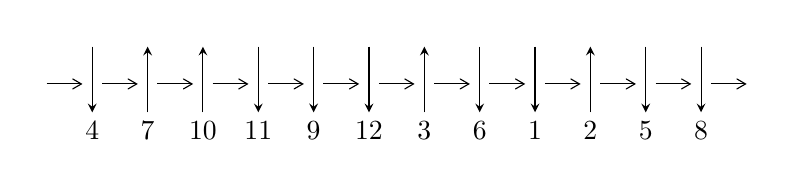
\begin{tikzpicture}[x=20pt, y=17pt]
	% nodes
	\node (C0) at (0, 0) {};
	\node (C1) at (1, 0) {};
	\node (C1U) at (1, +1) {};
	\node (C1D) at (1, -1) {4};

	\node (C2) at (2, 0) {};
	\node (C2U) at (2, +1) {};
	\node (C2D) at (2, -1) {7};

	\node (C3) at (3, 0) {};
	\node (C3U) at (3, +1) {};
	\node (C3D) at (3, -1) {10};

	\node (C4) at (4, 0) {};
	\node (C4U) at (4, +1) {};
	\node (C4D) at (4, -1) {11};

	\node (C5) at (5, 0) {};
	\node (C5U) at (5, +1) {};
	\node (C5D) at (5, -1) {9};

	\node (C6) at (6, 0) {};
	\node (C6U) at (6, +1) {};
	\node (C6D) at (6, -1) {12};

	\node (C7) at (7, 0) {};
	\node (C7U) at (7, +1) {};
	\node (C7D) at (7, -1) {3};

	\node (C8) at (8, 0) {};
	\node (C8U) at (8, +1) {};
	\node (C8D) at (8, -1) {6};

	\node (C9) at (9, 0) {};
	\node (C9U) at (9, +1) {};
	\node (C9D) at (9, -1) {1};

	\node (C10) at (10, 0) {};
	\node (C10U) at (10, +1) {};
	\node (C10D) at (10, -1) {2};

	\node (C11) at (11, 0) {};
	\node (C11U) at (11, +1) {};
	\node (C11D) at (11, -1) {5};

	\node (C12) at (12, 0) {};
	\node (C12U) at (12, +1) {};
	\node (C12D) at (12, -1) {8};
	\node (C13) at (13, 0) {};

	% arrows
	\draw[->,>={angle 60}]
	(C0) edge (C1) (C1) edge (C2) (C2) edge (C3) (C3) edge (C4) (C4) edge (C5) (C5) edge (C6) (C6) edge (C7) (C7) edge (C8) (C8) edge (C9) (C9) edge (C10) (C10) edge (C11) (C11) edge (C12) (C12) edge (C13) ;	\draw[->,>=stealth]
	(C1U) edge (C1D) (C2D) edge (C2U) (C3D) edge (C3U) (C4U) edge (C4D) (C5U) edge (C5D) (C6U) edge (C6D) (C7D) edge (C7U) (C8U) edge (C8D) (C9U) edge (C9D) (C10D) edge (C10U) (C11U) edge (C11D) (C12U) edge (C12D) ;
	\end{tikzpicture} \\
\hhline{~~} \\& 
\textbf{Solving Sequence} \\ \cline{2-2} 
 &
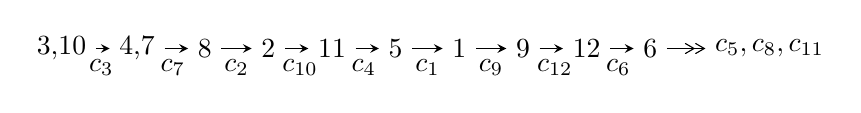
\begin{tikzpicture}[x=23pt, y=7pt]
	% node
	\node (A0) at (-1/8, 0) {3,10};
	\node (A1) at (17/16, 0) {4,7};
	\node (A2) at (17/8, 0) {8};
	\node (A3) at (25/8, 0) {2};
	\node (A4) at (33/8, 0) {11};
	\node (A5) at (41/8, 0) {5};
	\node (A6) at (49/8, 0) {1};
	\node (A7) at (57/8, 0) {9};
	\node (A8) at (65/8, 0) {12};
	\node (A9) at (73/8, 0) {6};
	\node (C1) at (1/2, -1) {$c_{3}$};
	\node (C2) at (13/8, -1) {$c_{7}$};
	\node (C3) at (21/8, -1) {$c_{2}$};
	\node (C4) at (29/8, -1) {$c_{10}$};
	\node (C5) at (37/8, -1) {$c_{4}$};
	\node (C6) at (45/8, -1) {$c_{1}$};
	\node (C7) at (53/8, -1) {$c_{9}$};
	\node (C8) at (61/8, -1) {$c_{12}$};
	\node (C9) at (69/8, -1) {$c_{6}$};
	\node (A10) at (11, 0) {$c_{5},c_{8},c_{11}$};

	% edge
	\draw[->,>=stealth]	
	(A0) edge (A1) (A1) edge (A2) (A2) edge (A3) (A3) edge (A4) (A4) edge (A5) (A5) edge (A6) (A6) edge (A7) (A7) edge (A8) (A8) edge (A9) ;
	\draw[->>,>={angle 60}]	
	(A9) edge (A10);
\end{tikzpicture} \\ 

\end{tabular} \\

\footnotetext{
The image of knot diagram is generated by the software ``\textbf{Draw programme}" developed by Andrew Bartholomew(\url{http://www.layer8.co.uk/maths/draw/index.htm\#Running-draw}), where we modified some parts for our purpose(\url{https://github.com/CATsTAILs/LinksPainter}).
}\phantom \\ \newline 
\centering \textbf{Ideals for irreducible components\footnotemark of $X_{\text{par}}$} 
 
\begin{align*}
I^u_{1}&=\langle 
-1.45606\times10^{1797} u^{172}+4.28745\times10^{1797} u^{171}+\cdots+9.44770\times10^{1797} b-2.86748\times10^{1798},\\
\phantom{I^u_{1}}&\phantom{= \langle  }1.34169\times10^{1798} u^{172}-3.67073\times10^{1798} u^{171}+\cdots+1.57462\times10^{1798} a+2.75924\times10^{1799},\\
\phantom{I^u_{1}}&\phantom{= \langle  }u^{173}-3 u^{172}+\cdots+74 u-5\rangle \\
I^u_{2}&=\langle 
-6.40598\times10^{90} u^{40}-1.88911\times10^{91} u^{39}+\cdots+3.54564\times10^{91} b+6.32745\times10^{91},\\
\phantom{I^u_{2}}&\phantom{= \langle  }3.86971\times10^{90} u^{40}+1.37761\times10^{91} u^{39}+\cdots+5.06521\times10^{90} a+2.20586\times10^{90},\;u^{41}+4 u^{40}+\cdots+8 u+1\rangle \\
\\
I^v_{1}&=\langle 
a,\;b-1,\;v-1\rangle \\
\end{align*}
\raggedright * 3 irreducible components of $\dim_{\mathbb{C}}=0$, with total 215 representations.\\
\footnotetext{All coefficients of polynomials are rational numbers. But the coefficients are sometimes approximated in decimal forms when there is not enough margin.}
\newpage
\renewcommand{\arraystretch}{1}
\centering \section*{I. $I^u_{1}= \langle -1.46\times10^{1797} u^{172}+4.29\times10^{1797} u^{171}+\cdots+9.45\times10^{1797} b-2.87\times10^{1798},\;1.34\times10^{1798} u^{172}-3.67\times10^{1798} u^{171}+\cdots+1.57\times10^{1798} a+2.76\times10^{1799},\;u^{173}-3 u^{172}+\cdots+74 u-5 \rangle$}
\flushleft \textbf{(i) Arc colorings}\\
\begin{tabular}{m{7pt} m{180pt} m{7pt} m{180pt} }
\flushright $a_{3}=$&$\begin{pmatrix}1\\0\end{pmatrix}$ \\
\flushright $a_{10}=$&$\begin{pmatrix}0\\u\end{pmatrix}$ \\
\flushright $a_{4}=$&$\begin{pmatrix}1\\- u^2\end{pmatrix}$ \\
\flushright $a_{7}=$&$\begin{pmatrix}-0.852074 u^{172}+2.33119 u^{171}+\cdots+192.061 u-17.5233\\0.154118 u^{172}-0.453809 u^{171}+\cdots-43.4524 u+3.03511\end{pmatrix}$ \\
\flushright $a_{8}=$&$\begin{pmatrix}-0.697956 u^{172}+1.87738 u^{171}+\cdots+148.609 u-14.4882\\0.154118 u^{172}-0.453809 u^{171}+\cdots-43.4524 u+3.03511\end{pmatrix}$ \\
\flushright $a_{2}=$&$\begin{pmatrix}0.880846 u^{172}-2.41344 u^{171}+\cdots-189.358 u+15.3554\\0.0527602 u^{172}-0.167734 u^{171}+\cdots-44.7616 u+7.47187\end{pmatrix}$ \\
\flushright $a_{11}=$&$\begin{pmatrix}0.659939 u^{172}-1.79682 u^{171}+\cdots-125.453 u+10.8685\\0.150489 u^{172}-0.412764 u^{171}+\cdots-33.4644 u+2.15245\end{pmatrix}$ \\
\flushright $a_{5}=$&$\begin{pmatrix}1.66068 u^{172}-4.55348 u^{171}+\cdots-348.176 u+32.1923\\-0.0936094 u^{172}+0.255286 u^{171}+\cdots+20.9243 u-1.12248\end{pmatrix}$ \\
\flushright $a_{1}=$&$\begin{pmatrix}0.990881 u^{172}-2.73865 u^{171}+\cdots-246.669 u+23.9728\\0.0504515 u^{172}-0.161358 u^{171}+\cdots-44.9493 u+7.44738\end{pmatrix}$ \\
\flushright $a_{9}=$&$\begin{pmatrix}1.14343 u^{172}-3.12968 u^{171}+\cdots-248.351 u+22.1620\\0.204142 u^{172}-0.568632 u^{171}+\cdots-60.6632 u+6.72298\end{pmatrix}$ \\
\flushright $a_{12}=$&$\begin{pmatrix}-0.911362 u^{172}+2.49693 u^{171}+\cdots+192.888 u-16.1126\\-0.100738 u^{172}+0.274420 u^{171}+\cdots+21.0835 u-2.10841\end{pmatrix}$ \\
\flushright $a_{6}=$&$\begin{pmatrix}0.642395 u^{172}-1.78447 u^{171}+\cdots-137.745 u+12.1505\\-0.0117123 u^{172}-0.00281222 u^{171}+\cdots-14.1390 u+1.15428\end{pmatrix}$\\&\end{tabular}
\flushleft \textbf{(ii) Obstruction class $= -1$}\\~\\
\flushleft \textbf{(iii) Cusp Shapes $= 4.49529 u^{172}-13.8680 u^{171}+\cdots-2310.57 u+192.724$}\\~\\
\newpage\renewcommand{\arraystretch}{1}
\flushleft \textbf{(iv) u-Polynomials at the component}\newline \\
\begin{tabular}{m{50pt}|m{274pt}}
Crossings & \hspace{64pt}u-Polynomials at each crossing \\
\hline $$\begin{aligned}c_{1}\end{aligned}$$&$\begin{aligned}
&u^{173}-19 u^{172}+\cdots+21313 u-34383
\end{aligned}$\\
\hline $$\begin{aligned}c_{2},c_{7}\end{aligned}$$&$\begin{aligned}
&u^{173}-2 u^{172}+\cdots-128 u-57
\end{aligned}$\\
\hline $$\begin{aligned}c_{3}\end{aligned}$$&$\begin{aligned}
&u^{173}-3 u^{172}+\cdots+74 u-5
\end{aligned}$\\
\hline $$\begin{aligned}c_{4},c_{11}\end{aligned}$$&$\begin{aligned}
&u^{173}-8 u^{172}+\cdots-475086499 u-26150301
\end{aligned}$\\
\hline $$\begin{aligned}c_{5},c_{8}\end{aligned}$$&$\begin{aligned}
&u^{173}-5 u^{172}+\cdots-39097 u+5255
\end{aligned}$\\
\hline $$\begin{aligned}c_{6}\end{aligned}$$&$\begin{aligned}
&u^{173}-2 u^{172}+\cdots-127187 u-8237
\end{aligned}$\\
\hline $$\begin{aligned}c_{9}\end{aligned}$$&$\begin{aligned}
&u^{173}-5 u^{172}+\cdots-11110439275 u-2018788719
\end{aligned}$\\
\hline $$\begin{aligned}c_{10}\end{aligned}$$&$\begin{aligned}
&u^{173}- u^{172}+\cdots-195900 u-10457
\end{aligned}$\\
\hline $$\begin{aligned}c_{12}\end{aligned}$$&$\begin{aligned}
&u^{173}+8 u^{172}+\cdots+109558 u-21897
\end{aligned}$\\
\hline
\end{tabular}\\~\\
\newpage\renewcommand{\arraystretch}{1}
\flushleft \textbf{(v) Riley Polynomials at the component}\newline \\
\begin{tabular}{m{50pt}|m{274pt}}
Crossings & \hspace{64pt}Riley Polynomials at each crossing \\
\hline $$\begin{aligned}c_{1}\end{aligned}$$&$\begin{aligned}
&y^{173}-51 y^{172}+\cdots+66157887691 y-1182190689
\end{aligned}$\\
\hline $$\begin{aligned}c_{2},c_{7}\end{aligned}$$&$\begin{aligned}
&y^{173}-84 y^{172}+\cdots+141898 y-3249
\end{aligned}$\\
\hline $$\begin{aligned}c_{3}\end{aligned}$$&$\begin{aligned}
&y^{173}+57 y^{172}+\cdots+226 y-25
\end{aligned}$\\
\hline $$\begin{aligned}c_{4},c_{11}\end{aligned}$$&$\begin{aligned}
&y^{173}-98 y^{172}+\cdots+14008959254796871 y-683838242390601
\end{aligned}$\\
\hline $$\begin{aligned}c_{5},c_{8}\end{aligned}$$&$\begin{aligned}
&y^{173}+93 y^{172}+\cdots-1610278131 y-27615025
\end{aligned}$\\
\hline $$\begin{aligned}c_{6}\end{aligned}$$&$\begin{aligned}
&y^{173}-10 y^{172}+\cdots+2537115305 y-67848169
\end{aligned}$\\
\hline $$\begin{aligned}c_{9}\end{aligned}$$&$\begin{aligned}
&y^{173}-55 y^{172}+\cdots-3.85\times10^{19} y-4.08\times10^{18}
\end{aligned}$\\
\hline $$\begin{aligned}c_{10}\end{aligned}$$&$\begin{aligned}
&y^{173}+53 y^{172}+\cdots+582535008 y-109348849
\end{aligned}$\\
\hline $$\begin{aligned}c_{12}\end{aligned}$$&$\begin{aligned}
&y^{173}-40 y^{172}+\cdots-18126440756 y-479478609
\end{aligned}$\\
\hline
\end{tabular}\\~\\
\newpage\flushleft \textbf{(vi) Complex Volumes and Cusp Shapes}
$$\begin{array}{c|c|c}  
\text{Solutions to }I^u_{1}& \I (\text{vol} + \sqrt{-1}CS) & \text{Cusp shape}\\
 \hline 
\begin{aligned}
u &= -0.771804 + 0.616839 I \\
a &= -0.39746 - 1.58134 I \\
b &= \phantom{-}0.575916 + 0.329596 I\end{aligned}
 & \phantom{-}0.73868 - 6.06646 I & \phantom{-0.000000 } 0 \\ \hline\begin{aligned}
u &= -0.771804 - 0.616839 I \\
a &= -0.39746 + 1.58134 I \\
b &= \phantom{-}0.575916 - 0.329596 I\end{aligned}
 & \phantom{-}0.73868 + 6.06646 I & \phantom{-0.000000 } 0 \\ \hline\begin{aligned}
u &= \phantom{-}0.327529 + 0.959841 I \\
a &= -0.909180 + 0.473505 I \\
b &= \phantom{-}0.521248 - 0.478347 I\end{aligned}
 & -4.82456 - 3.09167 I & \phantom{-0.000000 } 0 \\ \hline\begin{aligned}
u &= \phantom{-}0.327529 - 0.959841 I \\
a &= -0.909180 - 0.473505 I \\
b &= \phantom{-}0.521248 + 0.478347 I\end{aligned}
 & -4.82456 + 3.09167 I & \phantom{-0.000000 } 0 \\ \hline\begin{aligned}
u &= -0.893032 + 0.512926 I \\
a &= -1.87164 - 0.35247 I \\
b &= \phantom{-}1.195920 - 0.317103 I\end{aligned}
 & \phantom{-}3.46692 - 4.24825 I & \phantom{-0.000000 } 0 \\ \hline\begin{aligned}
u &= -0.893032 - 0.512926 I \\
a &= -1.87164 + 0.35247 I \\
b &= \phantom{-}1.195920 + 0.317103 I\end{aligned}
 & \phantom{-}3.46692 + 4.24825 I & \phantom{-0.000000 } 0 \\ \hline\begin{aligned}
u &= -0.884605 + 0.378784 I \\
a &= \phantom{-}1.85819 - 0.14668 I \\
b &= -1.265240 + 0.030420 I\end{aligned}
 & \phantom{-}7.57089 - 1.71431 I & \phantom{-0.000000 } 0 \\ \hline\begin{aligned}
u &= -0.884605 - 0.378784 I \\
a &= \phantom{-}1.85819 + 0.14668 I \\
b &= -1.265240 - 0.030420 I\end{aligned}
 & \phantom{-}7.57089 + 1.71431 I & \phantom{-0.000000 } 0 \\ \hline\begin{aligned}
u &= \phantom{-}1.020480 + 0.191153 I \\
a &= -2.22668 - 0.53281 I \\
b &= \phantom{-}1.060020 + 0.469899 I\end{aligned}
 & \phantom{-}2.47628 + 9.71556 I & \phantom{-0.000000 } 0 \\ \hline\begin{aligned}
u &= \phantom{-}1.020480 - 0.191153 I \\
a &= -2.22668 + 0.53281 I \\
b &= \phantom{-}1.060020 - 0.469899 I\end{aligned}
 & \phantom{-}2.47628 - 9.71556 I & \phantom{-0.000000 } 0\\
 \hline 
 \end{array}$$\newpage$$\begin{array}{c|c|c}  
\text{Solutions to }I^u_{1}& \I (\text{vol} + \sqrt{-1}CS) & \text{Cusp shape}\\
 \hline 
\begin{aligned}
u &= \phantom{-}0.310676 + 0.909070 I \\
a &= \phantom{-}1.13471 - 0.91152 I \\
b &= -0.769375 - 0.374994 I\end{aligned}
 & \phantom{-}1.35686 + 2.59200 I & \phantom{-0.000000 } 0 \\ \hline\begin{aligned}
u &= \phantom{-}0.310676 - 0.909070 I \\
a &= \phantom{-}1.13471 + 0.91152 I \\
b &= -0.769375 + 0.374994 I\end{aligned}
 & \phantom{-}1.35686 - 2.59200 I & \phantom{-0.000000 } 0 \\ \hline\begin{aligned}
u &= \phantom{-}0.209331 + 0.932459 I \\
a &= \phantom{-}0.515968 + 0.653908 I \\
b &= \phantom{-}0.891224 + 0.338281 I\end{aligned}
 & -1.01217 + 3.12518 I & \phantom{-0.000000 } 0 \\ \hline\begin{aligned}
u &= \phantom{-}0.209331 - 0.932459 I \\
a &= \phantom{-}0.515968 - 0.653908 I \\
b &= \phantom{-}0.891224 - 0.338281 I\end{aligned}
 & -1.01217 - 3.12518 I & \phantom{-0.000000 } 0 \\ \hline\begin{aligned}
u &= -0.903470 + 0.153525 I \\
a &= \phantom{-}0.089516 + 0.427393 I \\
b &= \phantom{-}0.150812 + 0.347980 I\end{aligned}
 & -1.85433 + 1.23746 I & \phantom{-0.000000 } 0 \\ \hline\begin{aligned}
u &= -0.903470 - 0.153525 I \\
a &= \phantom{-}0.089516 - 0.427393 I \\
b &= \phantom{-}0.150812 - 0.347980 I\end{aligned}
 & -1.85433 - 1.23746 I & \phantom{-0.000000 } 0 \\ \hline\begin{aligned}
u &= -0.534516 + 0.943325 I \\
a &= \phantom{-}0.253784 + 0.163165 I \\
b &= \phantom{-}0.143471 - 0.644994 I\end{aligned}
 & -5.23731 - 5.69130 I & \phantom{-0.000000 } 0 \\ \hline\begin{aligned}
u &= -0.534516 - 0.943325 I \\
a &= \phantom{-}0.253784 - 0.163165 I \\
b &= \phantom{-}0.143471 + 0.644994 I\end{aligned}
 & -5.23731 + 5.69130 I & \phantom{-0.000000 } 0 \\ \hline\begin{aligned}
u &= \phantom{-}0.847467 + 0.694335 I \\
a &= \phantom{-}1.130120 - 0.548135 I \\
b &= -1.074320 - 0.683913 I\end{aligned}
 & \phantom{-}2.13377 + 3.30366 I & \phantom{-0.000000 } 0 \\ \hline\begin{aligned}
u &= \phantom{-}0.847467 - 0.694335 I \\
a &= \phantom{-}1.130120 + 0.548135 I \\
b &= -1.074320 + 0.683913 I\end{aligned}
 & \phantom{-}2.13377 - 3.30366 I & \phantom{-0.000000 } 0\\
 \hline 
 \end{array}$$\newpage$$\begin{array}{c|c|c}  
\text{Solutions to }I^u_{1}& \I (\text{vol} + \sqrt{-1}CS) & \text{Cusp shape}\\
 \hline 
\begin{aligned}
u &= -1.059570 + 0.295085 I \\
a &= \phantom{-}1.94245 + 0.11465 I \\
b &= -1.155320 + 0.440201 I\end{aligned}
 & \phantom{-}6.18080 - 6.34984 I & \phantom{-0.000000 } 0 \\ \hline\begin{aligned}
u &= -1.059570 - 0.295085 I \\
a &= \phantom{-}1.94245 - 0.11465 I \\
b &= -1.155320 - 0.440201 I\end{aligned}
 & \phantom{-}6.18080 + 6.34984 I & \phantom{-0.000000 } 0 \\ \hline\begin{aligned}
u &= -1.057830 + 0.417082 I \\
a &= \phantom{-}1.365150 + 0.034155 I \\
b &= -1.59091 + 0.12319 I\end{aligned}
 & \phantom{-}4.45701 - 9.89476 I & \phantom{-0.000000 } 0 \\ \hline\begin{aligned}
u &= -1.057830 - 0.417082 I \\
a &= \phantom{-}1.365150 - 0.034155 I \\
b &= -1.59091 - 0.12319 I\end{aligned}
 & \phantom{-}4.45701 + 9.89476 I & \phantom{-0.000000 } 0 \\ \hline\begin{aligned}
u &= \phantom{-}0.115228 + 0.839112 I \\
a &= -1.67477 + 0.38358 I \\
b &= -1.149070 + 0.528934 I\end{aligned}
 & -4.12366 - 3.97170 I & \phantom{-0.000000 } 0 \\ \hline\begin{aligned}
u &= \phantom{-}0.115228 - 0.839112 I \\
a &= -1.67477 - 0.38358 I \\
b &= -1.149070 - 0.528934 I\end{aligned}
 & -4.12366 + 3.97170 I & \phantom{-0.000000 } 0 \\ \hline\begin{aligned}
u &= \phantom{-}0.274378 + 0.797674 I \\
a &= -0.885026 - 0.966071 I \\
b &= -0.954736 - 0.435772 I\end{aligned}
 & \phantom{-}2.53247 + 7.27988 I & \phantom{-0.000000 } 0 \\ \hline\begin{aligned}
u &= \phantom{-}0.274378 - 0.797674 I \\
a &= -0.885026 + 0.966071 I \\
b &= -0.954736 + 0.435772 I\end{aligned}
 & \phantom{-}2.53247 - 7.27988 I & \phantom{-0.000000 } 0 \\ \hline\begin{aligned}
u &= \phantom{-}0.811488 + 0.839964 I \\
a &= -1.57035 + 1.08983 I \\
b &= \phantom{-}0.245624 + 0.756593 I\end{aligned}
 & -7.44936 - 0.53307 I & \phantom{-0.000000 } 0 \\ \hline\begin{aligned}
u &= \phantom{-}0.811488 - 0.839964 I \\
a &= -1.57035 - 1.08983 I \\
b &= \phantom{-}0.245624 - 0.756593 I\end{aligned}
 & -7.44936 + 0.53307 I & \phantom{-0.000000 } 0\\
 \hline 
 \end{array}$$\newpage$$\begin{array}{c|c|c}  
\text{Solutions to }I^u_{1}& \I (\text{vol} + \sqrt{-1}CS) & \text{Cusp shape}\\
 \hline 
\begin{aligned}
u &= -0.595608 + 1.013850 I \\
a &= -0.169753 + 0.015600 I \\
b &= \phantom{-}0.001884 + 0.755426 I\end{aligned}
 & -5.25176 - 2.86179 I & \phantom{-0.000000 } 0 \\ \hline\begin{aligned}
u &= -0.595608 - 1.013850 I \\
a &= -0.169753 - 0.015600 I \\
b &= \phantom{-}0.001884 - 0.755426 I\end{aligned}
 & -5.25176 + 2.86179 I & \phantom{-0.000000 } 0 \\ \hline\begin{aligned}
u &= \phantom{-}0.485744 + 0.665646 I \\
a &= \phantom{-}1.006990 - 0.543825 I \\
b &= -1.25260 - 0.86382 I\end{aligned}
 & \phantom{-}0.02523 + 12.00230 I & \phantom{-0.000000 } 0 \\ \hline\begin{aligned}
u &= \phantom{-}0.485744 - 0.665646 I \\
a &= \phantom{-}1.006990 + 0.543825 I \\
b &= -1.25260 + 0.86382 I\end{aligned}
 & \phantom{-}0.02523 - 12.00230 I & \phantom{-0.000000 } 0 \\ \hline\begin{aligned}
u &= -0.288924 + 0.768932 I \\
a &= -1.45194 + 0.66827 I \\
b &= -0.568154 - 0.388478 I\end{aligned}
 & -4.58612 - 2.13205 I & \phantom{-0.000000 } 0 \\ \hline\begin{aligned}
u &= -0.288924 - 0.768932 I \\
a &= -1.45194 - 0.66827 I \\
b &= -0.568154 + 0.388478 I\end{aligned}
 & -4.58612 + 2.13205 I & \phantom{-0.000000 } 0 \\ \hline\begin{aligned}
u &= \phantom{-}0.090615 + 0.816399 I \\
a &= \phantom{-}1.34471 + 1.06956 I \\
b &= \phantom{-}0.693540 + 0.393354 I\end{aligned}
 & -3.40908 + 3.07298 I & \phantom{-0.000000 } 0 \\ \hline\begin{aligned}
u &= \phantom{-}0.090615 - 0.816399 I \\
a &= \phantom{-}1.34471 - 1.06956 I \\
b &= \phantom{-}0.693540 - 0.393354 I\end{aligned}
 & -3.40908 - 3.07298 I & \phantom{-0.000000 } 0 \\ \hline\begin{aligned}
u &= \phantom{-}0.656834 + 0.456210 I \\
a &= \phantom{-}2.44343 - 0.66596 I \\
b &= -0.020467 - 0.688172 I\end{aligned}
 & -3.03193 + 6.49857 I & \phantom{-0.000000 } 0 \\ \hline\begin{aligned}
u &= \phantom{-}0.656834 - 0.456210 I \\
a &= \phantom{-}2.44343 + 0.66596 I \\
b &= -0.020467 + 0.688172 I\end{aligned}
 & -3.03193 - 6.49857 I & \phantom{-0.000000 } 0\\
 \hline 
 \end{array}$$\newpage$$\begin{array}{c|c|c}  
\text{Solutions to }I^u_{1}& \I (\text{vol} + \sqrt{-1}CS) & \text{Cusp shape}\\
 \hline 
\begin{aligned}
u &= \phantom{-}0.573018 + 0.543113 I \\
a &= -1.036760 + 0.596641 I \\
b &= \phantom{-}1.14168 + 0.89708 I\end{aligned}
 & -2.74658 + 6.71616 I & \phantom{-0.000000 } 0 \\ \hline\begin{aligned}
u &= \phantom{-}0.573018 - 0.543113 I \\
a &= -1.036760 - 0.596641 I \\
b &= \phantom{-}1.14168 - 0.89708 I\end{aligned}
 & -2.74658 - 6.71616 I & \phantom{-0.000000 } 0 \\ \hline\begin{aligned}
u &= -1.050190 + 0.606462 I \\
a &= -1.38501 - 0.32197 I \\
b &= \phantom{-}1.53027 - 0.37409 I\end{aligned}
 & \phantom{-}2.82769 - 3.81698 I & \phantom{-0.000000 } 0 \\ \hline\begin{aligned}
u &= -1.050190 - 0.606462 I \\
a &= -1.38501 + 0.32197 I \\
b &= \phantom{-}1.53027 + 0.37409 I\end{aligned}
 & \phantom{-}2.82769 + 3.81698 I & \phantom{-0.000000 } 0 \\ \hline\begin{aligned}
u &= -0.620347 + 1.051040 I \\
a &= \phantom{-}0.111676 + 0.732193 I \\
b &= -1.253110 - 0.353916 I\end{aligned}
 & \phantom{-}0.75493 - 2.23733 I & \phantom{-0.000000 } 0 \\ \hline\begin{aligned}
u &= -0.620347 - 1.051040 I \\
a &= \phantom{-}0.111676 - 0.732193 I \\
b &= -1.253110 + 0.353916 I\end{aligned}
 & \phantom{-}0.75493 + 2.23733 I & \phantom{-0.000000 } 0 \\ \hline\begin{aligned}
u &= \phantom{-}0.798891 + 0.934167 I \\
a &= \phantom{-}1.73060 - 0.88718 I \\
b &= -1.085620 - 0.539353 I\end{aligned}
 & -4.08066 + 7.63216 I & \phantom{-0.000000 } 0 \\ \hline\begin{aligned}
u &= \phantom{-}0.798891 - 0.934167 I \\
a &= \phantom{-}1.73060 + 0.88718 I \\
b &= -1.085620 + 0.539353 I\end{aligned}
 & -4.08066 - 7.63216 I & \phantom{-0.000000 } 0 \\ \hline\begin{aligned}
u &= -0.436532 + 0.635112 I \\
a &= -1.38475 - 1.10083 I \\
b &= \phantom{-}1.237080 - 0.610945 I\end{aligned}
 & \phantom{-}3.24345 - 7.96682 I & \phantom{-0.000000 } 0 \\ \hline\begin{aligned}
u &= -0.436532 - 0.635112 I \\
a &= -1.38475 + 1.10083 I \\
b &= \phantom{-}1.237080 + 0.610945 I\end{aligned}
 & \phantom{-}3.24345 + 7.96682 I & \phantom{-0.000000 } 0\\
 \hline 
 \end{array}$$\newpage$$\begin{array}{c|c|c}  
\text{Solutions to }I^u_{1}& \I (\text{vol} + \sqrt{-1}CS) & \text{Cusp shape}\\
 \hline 
\begin{aligned}
u &= -0.476347 + 1.142860 I \\
a &= -0.248989 + 0.082084 I \\
b &= -0.371624 - 0.514992 I\end{aligned}
 & -6.14067 - 3.17595 I & \phantom{-0.000000 } 0 \\ \hline\begin{aligned}
u &= -0.476347 - 1.142860 I \\
a &= -0.248989 - 0.082084 I \\
b &= -0.371624 + 0.514992 I\end{aligned}
 & -6.14067 + 3.17595 I & \phantom{-0.000000 } 0 \\ \hline\begin{aligned}
u &= \phantom{-}1.201370 + 0.302411 I \\
a &= \phantom{-}1.301830 + 0.096557 I \\
b &= -1.261640 + 0.068574 I\end{aligned}
 & \phantom{-}3.90299 + 0.46319 I & \phantom{-0.000000 } 0 \\ \hline\begin{aligned}
u &= \phantom{-}1.201370 - 0.302411 I \\
a &= \phantom{-}1.301830 - 0.096557 I \\
b &= -1.261640 - 0.068574 I\end{aligned}
 & \phantom{-}3.90299 - 0.46319 I & \phantom{-0.000000 } 0 \\ \hline\begin{aligned}
u &= \phantom{-}0.790408 + 0.974551 I \\
a &= -0.222631 + 0.218548 I \\
b &= \phantom{-}0.570108 - 0.583458 I\end{aligned}
 & \phantom{-}1.39173 + 3.03834 I & \phantom{-0.000000 } 0 \\ \hline\begin{aligned}
u &= \phantom{-}0.790408 - 0.974551 I \\
a &= -0.222631 - 0.218548 I \\
b &= \phantom{-}0.570108 + 0.583458 I\end{aligned}
 & \phantom{-}1.39173 - 3.03834 I & \phantom{-0.000000 } 0 \\ \hline\begin{aligned}
u &= \phantom{-}0.652253 + 0.358586 I \\
a &= \phantom{-}0.351804 - 0.584101 I \\
b &= -0.082947 + 0.626679 I\end{aligned}
 & \phantom{-}3.14829 + 2.27443 I & \phantom{-0.000000 } 0 \\ \hline\begin{aligned}
u &= \phantom{-}0.652253 - 0.358586 I \\
a &= \phantom{-}0.351804 + 0.584101 I \\
b &= -0.082947 - 0.626679 I\end{aligned}
 & \phantom{-}3.14829 - 2.27443 I & \phantom{-0.000000 } 0 \\ \hline\begin{aligned}
u &= \phantom{-}1.090420 + 0.641267 I \\
a &= \phantom{-}1.28188 - 0.96977 I \\
b &= -0.951554 - 0.253556 I\end{aligned}
 & \phantom{-}0.79136 + 3.29959 I & \phantom{-0.000000 } 0 \\ \hline\begin{aligned}
u &= \phantom{-}1.090420 - 0.641267 I \\
a &= \phantom{-}1.28188 + 0.96977 I \\
b &= -0.951554 + 0.253556 I\end{aligned}
 & \phantom{-}0.79136 - 3.29959 I & \phantom{-0.000000 } 0\\
 \hline 
 \end{array}$$\newpage$$\begin{array}{c|c|c}  
\text{Solutions to }I^u_{1}& \I (\text{vol} + \sqrt{-1}CS) & \text{Cusp shape}\\
 \hline 
\begin{aligned}
u &= \phantom{-}1.192030 + 0.440347 I \\
a &= -1.231700 - 0.113799 I \\
b &= \phantom{-}1.301890 - 0.116928 I\end{aligned}
 & \phantom{-}7.48423 + 5.34721 I & \phantom{-0.000000 } 0 \\ \hline\begin{aligned}
u &= \phantom{-}1.192030 - 0.440347 I \\
a &= -1.231700 + 0.113799 I \\
b &= \phantom{-}1.301890 + 0.116928 I\end{aligned}
 & \phantom{-}7.48423 - 5.34721 I & \phantom{-0.000000 } 0 \\ \hline\begin{aligned}
u &= \phantom{-}0.781611 + 1.011340 I \\
a &= \phantom{-}0.088109 + 0.454713 I \\
b &= \phantom{-}0.965838 - 0.735415 I\end{aligned}
 & \phantom{-}1.33379 + 2.59811 I & \phantom{-0.000000 } 0 \\ \hline\begin{aligned}
u &= \phantom{-}0.781611 - 1.011340 I \\
a &= \phantom{-}0.088109 - 0.454713 I \\
b &= \phantom{-}0.965838 + 0.735415 I\end{aligned}
 & \phantom{-}1.33379 - 2.59811 I & \phantom{-0.000000 } 0 \\ \hline\begin{aligned}
u &= -0.898132 + 0.938994 I \\
a &= -0.113394 + 0.229786 I \\
b &= \phantom{-}0.300953 + 0.965635 I\end{aligned}
 & -2.29687 - 3.81092 I & \phantom{-0.000000 } 0 \\ \hline\begin{aligned}
u &= -0.898132 - 0.938994 I \\
a &= -0.113394 - 0.229786 I \\
b &= \phantom{-}0.300953 - 0.965635 I\end{aligned}
 & -2.29687 + 3.81092 I & \phantom{-0.000000 } 0 \\ \hline\begin{aligned}
u &= -0.202556 + 0.666398 I \\
a &= \phantom{-}1.48907 - 2.53927 I \\
b &= \phantom{-}1.144620 - 0.491821 I\end{aligned}
 & -0.04009 - 10.77620 I & \phantom{-0.000000 } 0 \\ \hline\begin{aligned}
u &= -0.202556 - 0.666398 I \\
a &= \phantom{-}1.48907 + 2.53927 I \\
b &= \phantom{-}1.144620 + 0.491821 I\end{aligned}
 & -0.04009 + 10.77620 I & \phantom{-0.000000 } 0 \\ \hline\begin{aligned}
u &= -0.582427 + 1.198980 I \\
a &= \phantom{-}0.1062270 + 0.0814320 I \\
b &= \phantom{-}0.307299 + 0.661890 I\end{aligned}
 & -5.39810 - 6.59757 I & \phantom{-0.000000 } 0 \\ \hline\begin{aligned}
u &= -0.582427 - 1.198980 I \\
a &= \phantom{-}0.1062270 - 0.0814320 I \\
b &= \phantom{-}0.307299 - 0.661890 I\end{aligned}
 & -5.39810 + 6.59757 I & \phantom{-0.000000 } 0\\
 \hline 
 \end{array}$$\newpage$$\begin{array}{c|c|c}  
\text{Solutions to }I^u_{1}& \I (\text{vol} + \sqrt{-1}CS) & \text{Cusp shape}\\
 \hline 
\begin{aligned}
u &= -0.595071 + 0.293276 I \\
a &= -0.960088 - 0.059502 I \\
b &= \phantom{-}1.157920 - 0.699124 I\end{aligned}
 & -2.76594 - 0.82042 I & \phantom{-0.000000 } 0 \\ \hline\begin{aligned}
u &= -0.595071 - 0.293276 I \\
a &= -0.960088 + 0.059502 I \\
b &= \phantom{-}1.157920 + 0.699124 I\end{aligned}
 & -2.76594 + 0.82042 I & \phantom{-0.000000 } 0 \\ \hline\begin{aligned}
u &= \phantom{-}0.197798 + 0.632612 I \\
a &= \phantom{-}0.298551 + 0.201969 I \\
b &= -0.140312 - 0.490544 I\end{aligned}
 & -0.251995 + 1.167390 I & \phantom{-0.000000 } 0 \\ \hline\begin{aligned}
u &= \phantom{-}0.197798 - 0.632612 I \\
a &= \phantom{-}0.298551 - 0.201969 I \\
b &= -0.140312 + 0.490544 I\end{aligned}
 & -0.251995 - 1.167390 I & \phantom{-0.000000 } 0 \\ \hline\begin{aligned}
u &= -1.176470 + 0.663942 I \\
a &= -1.026570 - 0.199156 I \\
b &= \phantom{-}1.038940 - 0.525323 I\end{aligned}
 & -3.18652 - 1.20243 I & \phantom{-0.000000 } 0 \\ \hline\begin{aligned}
u &= -1.176470 - 0.663942 I \\
a &= -1.026570 + 0.199156 I \\
b &= \phantom{-}1.038940 + 0.525323 I\end{aligned}
 & -3.18652 + 1.20243 I & \phantom{-0.000000 } 0 \\ \hline\begin{aligned}
u &= \phantom{-}0.489322 + 0.424466 I \\
a &= \phantom{-}3.61572 - 1.51104 I \\
b &= -1.041160 - 0.486793 I\end{aligned}
 & -2.98959 + 5.99414 I & \phantom{-0.000000 } 0 \\ \hline\begin{aligned}
u &= \phantom{-}0.489322 - 0.424466 I \\
a &= \phantom{-}3.61572 + 1.51104 I \\
b &= -1.041160 + 0.486793 I\end{aligned}
 & -2.98959 - 5.99414 I & \phantom{-0.000000 } 0 \\ \hline\begin{aligned}
u &= \phantom{-}0.553755 + 0.311828 I \\
a &= \phantom{-}0.086698 + 0.147270 I \\
b &= \phantom{-}0.00775 - 1.58504 I\end{aligned}
 & -2.77098 - 3.15696 I & \phantom{-0.000000 } 0 \\ \hline\begin{aligned}
u &= \phantom{-}0.553755 - 0.311828 I \\
a &= \phantom{-}0.086698 - 0.147270 I \\
b &= \phantom{-}0.00775 + 1.58504 I\end{aligned}
 & -2.77098 + 3.15696 I & \phantom{-0.000000 } 0\\
 \hline 
 \end{array}$$\newpage$$\begin{array}{c|c|c}  
\text{Solutions to }I^u_{1}& \I (\text{vol} + \sqrt{-1}CS) & \text{Cusp shape}\\
 \hline 
\begin{aligned}
u &= \phantom{-}1.051630 + 0.871791 I \\
a &= \phantom{-}1.47913 - 0.77264 I \\
b &= -0.396452 - 0.582440 I\end{aligned}
 & -3.81059 - 7.12042 I & \phantom{-0.000000 } 0 \\ \hline\begin{aligned}
u &= \phantom{-}1.051630 - 0.871791 I \\
a &= \phantom{-}1.47913 + 0.77264 I \\
b &= -0.396452 + 0.582440 I\end{aligned}
 & -3.81059 + 7.12042 I & \phantom{-0.000000 } 0 \\ \hline\begin{aligned}
u &= \phantom{-}1.339450 + 0.272311 I \\
a &= -1.305310 - 0.185779 I \\
b &= \phantom{-}1.224180 - 0.120179 I\end{aligned}
 & \phantom{-}7.83078 - 4.10815 I & \phantom{-0.000000 } 0 \\ \hline\begin{aligned}
u &= \phantom{-}1.339450 - 0.272311 I \\
a &= -1.305310 + 0.185779 I \\
b &= \phantom{-}1.224180 + 0.120179 I\end{aligned}
 & \phantom{-}7.83078 + 4.10815 I & \phantom{-0.000000 } 0 \\ \hline\begin{aligned}
u &= -0.260548 + 1.346570 I \\
a &= -0.372320 + 0.129068 I \\
b &= \phantom{-}0.383847 - 0.198499 I\end{aligned}
 & -5.78719 - 3.27740 I & \phantom{-0.000000 } 0 \\ \hline\begin{aligned}
u &= -0.260548 - 1.346570 I \\
a &= -0.372320 - 0.129068 I \\
b &= \phantom{-}0.383847 + 0.198499 I\end{aligned}
 & -5.78719 + 3.27740 I & \phantom{-0.000000 } 0 \\ \hline\begin{aligned}
u &= -0.540444 + 0.236092 I \\
a &= -1.76684 - 1.87855 I \\
b &= \phantom{-}1.064290 - 0.461952 I\end{aligned}
 & \phantom{-}6.03952 - 1.30060 I & \phantom{-0.000000 } 0 \\ \hline\begin{aligned}
u &= -0.540444 - 0.236092 I \\
a &= -1.76684 + 1.87855 I \\
b &= \phantom{-}1.064290 + 0.461952 I\end{aligned}
 & \phantom{-}6.03952 + 1.30060 I & \phantom{-0.000000 } 0 \\ \hline\begin{aligned}
u &= \phantom{-}1.00260 + 0.99784 I \\
a &= -0.0479860 + 0.0683654 I \\
b &= \phantom{-}0.463303 - 1.175820 I\end{aligned}
 & -3.9091 + 14.3052 I & \phantom{-0.000000 } 0 \\ \hline\begin{aligned}
u &= \phantom{-}1.00260 - 0.99784 I \\
a &= -0.0479860 - 0.0683654 I \\
b &= \phantom{-}0.463303 + 1.175820 I\end{aligned}
 & -3.9091 - 14.3052 I & \phantom{-0.000000 } 0\\
 \hline 
 \end{array}$$\newpage$$\begin{array}{c|c|c}  
\text{Solutions to }I^u_{1}& \I (\text{vol} + \sqrt{-1}CS) & \text{Cusp shape}\\
 \hline 
\begin{aligned}
u &= -0.380777 + 0.433816 I \\
a &= \phantom{-}1.39771 + 1.44587 I \\
b &= -1.141210 + 0.620104 I\end{aligned}
 & \phantom{-}1.18248 - 3.63276 I & \phantom{-0.000000 } 0 \\ \hline\begin{aligned}
u &= -0.380777 - 0.433816 I \\
a &= \phantom{-}1.39771 - 1.44587 I \\
b &= -1.141210 - 0.620104 I\end{aligned}
 & \phantom{-}1.18248 + 3.63276 I & \phantom{-0.000000 } 0 \\ \hline\begin{aligned}
u &= \phantom{-}1.02110 + 0.99823 I \\
a &= \phantom{-}0.0181824 - 0.0903520 I \\
b &= -0.565972 + 1.238050 I\end{aligned}
 & -7.12079 + 7.64482 I & \phantom{-0.000000 } 0 \\ \hline\begin{aligned}
u &= \phantom{-}1.02110 - 0.99823 I \\
a &= \phantom{-}0.0181824 + 0.0903520 I \\
b &= -0.565972 - 1.238050 I\end{aligned}
 & -7.12079 - 7.64482 I & \phantom{-0.000000 } 0 \\ \hline\begin{aligned}
u &= -0.221479 + 0.524398 I \\
a &= \phantom{-}0.420856 - 0.196728 I \\
b &= -0.073568 - 1.045510 I\end{aligned}
 & -0.32442 + 2.05901 I & \phantom{-0.000000 } 0 \\ \hline\begin{aligned}
u &= -0.221479 - 0.524398 I \\
a &= \phantom{-}0.420856 + 0.196728 I \\
b &= -0.073568 + 1.045510 I\end{aligned}
 & -0.32442 - 2.05901 I & \phantom{-0.000000 } 0 \\ \hline\begin{aligned}
u &= -0.94557 + 1.07962 I \\
a &= \phantom{-}0.069344 - 0.261082 I \\
b &= -0.341921 - 0.882790 I\end{aligned}
 & \phantom{-}1.76439 - 8.64944 I & \phantom{-0.000000 } 0 \\ \hline\begin{aligned}
u &= -0.94557 - 1.07962 I \\
a &= \phantom{-}0.069344 + 0.261082 I \\
b &= -0.341921 + 0.882790 I\end{aligned}
 & \phantom{-}1.76439 + 8.64944 I & \phantom{-0.000000 } 0 \\ \hline\begin{aligned}
u &= \phantom{-}0.01118 + 1.43980 I \\
a &= \phantom{-}0.077941 - 0.361287 I \\
b &= \phantom{-}1.150280 - 0.237849 I\end{aligned}
 & \phantom{-}0.01971 + 4.42792 I & \phantom{-0.000000 } 0 \\ \hline\begin{aligned}
u &= \phantom{-}0.01118 - 1.43980 I \\
a &= \phantom{-}0.077941 + 0.361287 I \\
b &= \phantom{-}1.150280 + 0.237849 I\end{aligned}
 & \phantom{-}0.01971 - 4.42792 I & \phantom{-0.000000 } 0\\
 \hline 
 \end{array}$$\newpage$$\begin{array}{c|c|c}  
\text{Solutions to }I^u_{1}& \I (\text{vol} + \sqrt{-1}CS) & \text{Cusp shape}\\
 \hline 
\begin{aligned}
u &= \phantom{-}0.89322 + 1.14294 I \\
a &= -1.42783 + 0.82370 I \\
b &= \phantom{-}1.110460 + 0.566366 I\end{aligned}
 & -3.14263 + 11.42110 I & \phantom{-0.000000 } 0 \\ \hline\begin{aligned}
u &= \phantom{-}0.89322 - 1.14294 I \\
a &= -1.42783 - 0.82370 I \\
b &= \phantom{-}1.110460 - 0.566366 I\end{aligned}
 & -3.14263 - 11.42110 I & \phantom{-0.000000 } 0 \\ \hline\begin{aligned}
u &= -1.01855 + 1.06509 I \\
a &= -1.34401 - 0.89192 I \\
b &= \phantom{-}1.079310 - 0.862048 I\end{aligned}
 & \phantom{-}1.61273 - 9.07333 I & \phantom{-0.000000 } 0 \\ \hline\begin{aligned}
u &= -1.01855 - 1.06509 I \\
a &= -1.34401 + 0.89192 I \\
b &= \phantom{-}1.079310 + 0.862048 I\end{aligned}
 & \phantom{-}1.61273 + 9.07333 I & \phantom{-0.000000 } 0 \\ \hline\begin{aligned}
u &= -1.07007 + 1.01607 I \\
a &= \phantom{-}0.222969 - 0.283585 I \\
b &= -0.588593 - 0.899615 I\end{aligned}
 & \phantom{-}1.93016 + 1.77297 I & \phantom{-0.000000 } 0 \\ \hline\begin{aligned}
u &= -1.07007 - 1.01607 I \\
a &= \phantom{-}0.222969 + 0.283585 I \\
b &= -0.588593 + 0.899615 I\end{aligned}
 & \phantom{-}1.93016 - 1.77297 I & \phantom{-0.000000 } 0 \\ \hline\begin{aligned}
u &= -0.59580 + 1.36183 I \\
a &= \phantom{-}0.330826 + 0.187193 I \\
b &= -0.412461 - 0.047465 I\end{aligned}
 & -5.08049 - 6.03903 I & \phantom{-0.000000 } 0 \\ \hline\begin{aligned}
u &= -0.59580 - 1.36183 I \\
a &= \phantom{-}0.330826 - 0.187193 I \\
b &= -0.412461 + 0.047465 I\end{aligned}
 & -5.08049 + 6.03903 I & \phantom{-0.000000 } 0 \\ \hline\begin{aligned}
u &= -1.25785 + 0.80648 I \\
a &= -1.60637 - 0.35517 I \\
b &= \phantom{-}0.929722 - 0.430484 I\end{aligned}
 & \phantom{-}2.25673 - 6.96320 I & \phantom{-0.000000 } 0 \\ \hline\begin{aligned}
u &= -1.25785 - 0.80648 I \\
a &= -1.60637 + 0.35517 I \\
b &= \phantom{-}0.929722 + 0.430484 I\end{aligned}
 & \phantom{-}2.25673 + 6.96320 I & \phantom{-0.000000 } 0\\
 \hline 
 \end{array}$$\newpage$$\begin{array}{c|c|c}  
\text{Solutions to }I^u_{1}& \I (\text{vol} + \sqrt{-1}CS) & \text{Cusp shape}\\
 \hline 
\begin{aligned}
u &= -0.68933 + 1.33561 I \\
a &= -1.32515 - 1.00348 I \\
b &= \phantom{-}0.845483 - 0.389760 I\end{aligned}
 & \phantom{-}2.07173 - 0.49277 I & \phantom{-0.000000 } 0 \\ \hline\begin{aligned}
u &= -0.68933 - 1.33561 I \\
a &= -1.32515 + 1.00348 I \\
b &= \phantom{-}0.845483 + 0.389760 I\end{aligned}
 & \phantom{-}2.07173 + 0.49277 I & \phantom{-0.000000 } 0 \\ \hline\begin{aligned}
u &= -0.026810 + 0.492713 I \\
a &= \phantom{-}1.094720 + 0.033699 I \\
b &= -1.46826 + 0.52395 I\end{aligned}
 & -1.06608 + 2.76062 I & -21.2259 - 6.9158 I \\ \hline\begin{aligned}
u &= -0.026810 - 0.492713 I \\
a &= \phantom{-}1.094720 - 0.033699 I \\
b &= -1.46826 - 0.52395 I\end{aligned}
 & -1.06608 - 2.76062 I & -21.2259 + 6.9158 I \\ \hline\begin{aligned}
u &= \phantom{-}0.29341 + 1.47990 I \\
a &= -0.39388 + 1.47257 I \\
b &= -0.00064 + 1.43127 I\end{aligned}
 & -7.83616 - 0.90984 I & \phantom{-0.000000 } 0 \\ \hline\begin{aligned}
u &= \phantom{-}0.29341 - 1.47990 I \\
a &= -0.39388 - 1.47257 I \\
b &= -0.00064 - 1.43127 I\end{aligned}
 & -7.83616 + 0.90984 I & \phantom{-0.000000 } 0 \\ \hline\begin{aligned}
u &= -0.219019 + 0.426393 I \\
a &= -1.36079 - 2.17280 I \\
b &= -0.390412 + 0.560000 I\end{aligned}
 & \phantom{-}0.15969 - 6.71976 I & -4.00000 + 5.95672 I \\ \hline\begin{aligned}
u &= -0.219019 - 0.426393 I \\
a &= -1.36079 + 2.17280 I \\
b &= -0.390412 - 0.560000 I\end{aligned}
 & \phantom{-}0.15969 + 6.71976 I & -4.00000 - 5.95672 I \\ \hline\begin{aligned}
u &= \phantom{-}1.26696 + 0.87132 I \\
a &= \phantom{-}1.55381 - 0.28865 I \\
b &= -1.136610 - 0.482113 I\end{aligned}
 & -2.21266 + 9.70416 I & \phantom{-0.000000 } 0 \\ \hline\begin{aligned}
u &= \phantom{-}1.26696 - 0.87132 I \\
a &= \phantom{-}1.55381 + 0.28865 I \\
b &= -1.136610 + 0.482113 I\end{aligned}
 & -2.21266 - 9.70416 I & \phantom{-0.000000 } 0\\
 \hline 
 \end{array}$$\newpage$$\begin{array}{c|c|c}  
\text{Solutions to }I^u_{1}& \I (\text{vol} + \sqrt{-1}CS) & \text{Cusp shape}\\
 \hline 
\begin{aligned}
u &= -0.70912 + 1.39026 I \\
a &= \phantom{-}0.529659 - 0.194908 I \\
b &= -0.858036 - 0.602660 I\end{aligned}
 & \phantom{-}1.25833 + 1.46506 I & \phantom{-0.000000 } 0 \\ \hline\begin{aligned}
u &= -0.70912 - 1.39026 I \\
a &= \phantom{-}0.529659 + 0.194908 I \\
b &= -0.858036 + 0.602660 I\end{aligned}
 & \phantom{-}1.25833 - 1.46506 I & \phantom{-0.000000 } 0 \\ \hline\begin{aligned}
u &= \phantom{-}0.74538 + 1.37969 I \\
a &= \phantom{-}0.779922 - 0.083463 I \\
b &= -0.690066 + 0.410656 I\end{aligned}
 & -3.45403 + 0.99244 I & \phantom{-0.000000 } 0 \\ \hline\begin{aligned}
u &= \phantom{-}0.74538 - 1.37969 I \\
a &= \phantom{-}0.779922 + 0.083463 I \\
b &= -0.690066 - 0.410656 I\end{aligned}
 & -3.45403 - 0.99244 I & \phantom{-0.000000 } 0 \\ \hline\begin{aligned}
u &= \phantom{-}0.270858 + 0.299713 I \\
a &= -0.42510 - 3.44166 I \\
b &= -1.120710 - 0.431374 I\end{aligned}
 & \phantom{-}2.61891 - 2.60527 I & \phantom{-}2.19979 + 2.42977 I \\ \hline\begin{aligned}
u &= \phantom{-}0.270858 - 0.299713 I \\
a &= -0.42510 + 3.44166 I \\
b &= -1.120710 + 0.431374 I\end{aligned}
 & \phantom{-}2.61891 + 2.60527 I & \phantom{-}2.19979 - 2.42977 I \\ \hline\begin{aligned}
u &= \phantom{-}1.19735 + 1.05685 I \\
a &= -1.40190 + 0.42418 I \\
b &= \phantom{-}1.165460 + 0.514043 I\end{aligned}
 & -2.14917 + 7.43905 I & \phantom{-0.000000 } 0 \\ \hline\begin{aligned}
u &= \phantom{-}1.19735 - 1.05685 I \\
a &= -1.40190 - 0.42418 I \\
b &= \phantom{-}1.165460 - 0.514043 I\end{aligned}
 & -2.14917 - 7.43905 I & \phantom{-0.000000 } 0 \\ \hline\begin{aligned}
u &= \phantom{-}0.131695 + 0.359172 I \\
a &= -1.94861 + 4.86669 I \\
b &= \phantom{-}0.998265 + 0.422503 I\end{aligned}
 & -2.40329 + 0.40749 I & -11.27009 + 0.81722 I \\ \hline\begin{aligned}
u &= \phantom{-}0.131695 - 0.359172 I \\
a &= -1.94861 - 4.86669 I \\
b &= \phantom{-}0.998265 - 0.422503 I\end{aligned}
 & -2.40329 - 0.40749 I & -11.27009 - 0.81722 I\\
 \hline 
 \end{array}$$\newpage$$\begin{array}{c|c|c}  
\text{Solutions to }I^u_{1}& \I (\text{vol} + \sqrt{-1}CS) & \text{Cusp shape}\\
 \hline 
\begin{aligned}
u &= -1.14275 + 1.14857 I \\
a &= \phantom{-}1.24104 + 0.69121 I \\
b &= -1.23896 + 0.77805 I\end{aligned}
 & -4.8409 - 14.7640 I & \phantom{-0.000000 } 0 \\ \hline\begin{aligned}
u &= -1.14275 - 1.14857 I \\
a &= \phantom{-}1.24104 - 0.69121 I \\
b &= -1.23896 - 0.77805 I\end{aligned}
 & -4.8409 + 14.7640 I & \phantom{-0.000000 } 0 \\ \hline\begin{aligned}
u &= \phantom{-}0.61057 + 1.50821 I \\
a &= \phantom{-}0.412925 + 0.132575 I \\
b &= -0.797914 + 0.364812 I\end{aligned}
 & -1.292400 + 0.235559 I & \phantom{-0.000000 } 0 \\ \hline\begin{aligned}
u &= \phantom{-}0.61057 - 1.50821 I \\
a &= \phantom{-}0.412925 - 0.132575 I \\
b &= -0.797914 - 0.364812 I\end{aligned}
 & -1.292400 - 0.235559 I & \phantom{-0.000000 } 0 \\ \hline\begin{aligned}
u &= \phantom{-}0.360748 + 0.057808 I \\
a &= -1.81412 - 2.11052 I \\
b &= \phantom{-}0.322395 - 1.000550 I\end{aligned}
 & -5.45575 - 3.27553 I & -11.12246 + 3.81811 I \\ \hline\begin{aligned}
u &= \phantom{-}0.360748 - 0.057808 I \\
a &= -1.81412 + 2.11052 I \\
b &= \phantom{-}0.322395 + 1.000550 I\end{aligned}
 & -5.45575 + 3.27553 I & -11.12246 - 3.81811 I \\ \hline\begin{aligned}
u &= -1.18500 + 1.16023 I \\
a &= -1.252350 - 0.647899 I \\
b &= \phantom{-}1.23895 - 0.73568 I\end{aligned}
 & -1.4041 - 21.0729 I & \phantom{-0.000000 } 0 \\ \hline\begin{aligned}
u &= -1.18500 - 1.16023 I \\
a &= -1.252350 + 0.647899 I \\
b &= \phantom{-}1.23895 + 0.73568 I\end{aligned}
 & -1.4041 + 21.0729 I & \phantom{-0.000000 } 0 \\ \hline\begin{aligned}
u &= \phantom{-}0.229098 + 0.236735 I \\
a &= \phantom{-}4.67353 - 10.02870 I \\
b &= \phantom{-}0.417238 - 0.056129 I\end{aligned}
 & -3.21981 - 6.95231 I & -16.0662 + 21.3010 I \\ \hline\begin{aligned}
u &= \phantom{-}0.229098 - 0.236735 I \\
a &= \phantom{-}4.67353 + 10.02870 I \\
b &= \phantom{-}0.417238 + 0.056129 I\end{aligned}
 & -3.21981 + 6.95231 I & -16.0662 - 21.3010 I\\
 \hline 
 \end{array}$$\newpage$$\begin{array}{c|c|c}  
\text{Solutions to }I^u_{1}& \I (\text{vol} + \sqrt{-1}CS) & \text{Cusp shape}\\
 \hline 
\begin{aligned}
u &= -0.281786 + 0.164554 I \\
a &= -1.57933 - 3.60160 I \\
b &= -0.632665 - 0.429307 I\end{aligned}
 & \phantom{-}1.61418 - 3.63737 I & -3.03644 + 2.05493 I \\ \hline\begin{aligned}
u &= -0.281786 - 0.164554 I \\
a &= -1.57933 + 3.60160 I \\
b &= -0.632665 + 0.429307 I\end{aligned}
 & \phantom{-}1.61418 + 3.63737 I & -3.03644 - 2.05493 I \\ \hline\begin{aligned}
u &= -1.23998 + 1.15184 I \\
a &= \phantom{-}1.36064 + 0.54329 I \\
b &= -0.915621 + 0.418635 I\end{aligned}
 & -0.85773 - 3.62337 I & \phantom{-0.000000 } 0 \\ \hline\begin{aligned}
u &= -1.23998 - 1.15184 I \\
a &= \phantom{-}1.36064 - 0.54329 I \\
b &= -0.915621 - 0.418635 I\end{aligned}
 & -0.85773 + 3.62337 I & \phantom{-0.000000 } 0 \\ \hline\begin{aligned}
u &= -0.199861 + 0.231647 I \\
a &= \phantom{-}0.95907 + 3.00855 I \\
b &= \phantom{-}0.666540 + 0.257986 I\end{aligned}
 & -1.46465 - 0.07572 I & -7.82957 - 0.25967 I \\ \hline\begin{aligned}
u &= -0.199861 - 0.231647 I \\
a &= \phantom{-}0.95907 - 3.00855 I \\
b &= \phantom{-}0.666540 - 0.257986 I\end{aligned}
 & -1.46465 + 0.07572 I & -7.82957 + 0.25967 I \\ \hline\begin{aligned}
u &= \phantom{-}0.275213\phantom{ +0.000000I} \\
a &= -14.8178\phantom{ +0.000000I} \\
b &= -0.369430\phantom{ +0.000000I}\end{aligned}
 & -7.33542\phantom{ +0.000000I} & -36.0940\phantom{ +0.000000I} \\ \hline\begin{aligned}
u &= \phantom{-}1.23400 + 1.22259 I \\
a &= -1.144000 + 0.603249 I \\
b &= \phantom{-}1.173050 + 0.611089 I\end{aligned}
 & \phantom{-}0.34581 + 9.42252 I & \phantom{-0.000000 } 0 \\ \hline\begin{aligned}
u &= \phantom{-}1.23400 - 1.22259 I \\
a &= -1.144000 - 0.603249 I \\
b &= \phantom{-}1.173050 - 0.611089 I\end{aligned}
 & \phantom{-}0.34581 - 9.42252 I & \phantom{-0.000000 } 0 \\ \hline\begin{aligned}
u &= -1.44536 + 0.98520 I \\
a &= \phantom{-}1.143970 + 0.261724 I \\
b &= -0.985011 + 0.449323 I\end{aligned}
 & -2.45138 - 4.64512 I & \phantom{-0.000000 } 0\\
 \hline 
 \end{array}$$\newpage$$\begin{array}{c|c|c}  
\text{Solutions to }I^u_{1}& \I (\text{vol} + \sqrt{-1}CS) & \text{Cusp shape}\\
 \hline 
\begin{aligned}
u &= -1.44536 - 0.98520 I \\
a &= \phantom{-}1.143970 - 0.261724 I \\
b &= -0.985011 - 0.449323 I\end{aligned}
 & -2.45138 + 4.64512 I & \phantom{-0.000000 } 0 \\ \hline\begin{aligned}
u &= \phantom{-}0.233347 + 0.056878 I \\
a &= -1.75864 - 1.41813 I \\
b &= \phantom{-}1.47296 - 0.43619 I\end{aligned}
 & -1.73590 + 0.84771 I & \phantom{-}10.7047 - 12.7164 I \\ \hline\begin{aligned}
u &= \phantom{-}0.233347 - 0.056878 I \\
a &= -1.75864 + 1.41813 I \\
b &= \phantom{-}1.47296 + 0.43619 I\end{aligned}
 & -1.73590 - 0.84771 I & \phantom{-}10.7047 + 12.7164 I \\ \hline\begin{aligned}
u &= -0.161708 + 0.164950 I \\
a &= \phantom{-}0.039432 + 1.336790 I \\
b &= -0.675722 + 1.129920 I\end{aligned}
 & -0.73454 - 2.34093 I & \phantom{-}14.3158 - 10.9429 I \\ \hline\begin{aligned}
u &= -0.161708 - 0.164950 I \\
a &= \phantom{-}0.039432 - 1.336790 I \\
b &= -0.675722 - 1.129920 I\end{aligned}
 & -0.73454 + 2.34093 I & \phantom{-}14.3158 + 10.9429 I \\ \hline\begin{aligned}
u &= \phantom{-}1.35566 + 1.14725 I \\
a &= \phantom{-}1.062650 - 0.562680 I \\
b &= -1.188430 - 0.669605 I\end{aligned}
 & \phantom{-}3.94810 + 4.36162 I & \phantom{-0.000000 } 0 \\ \hline\begin{aligned}
u &= \phantom{-}1.35566 - 1.14725 I \\
a &= \phantom{-}1.062650 + 0.562680 I \\
b &= -1.188430 + 0.669605 I\end{aligned}
 & \phantom{-}3.94810 - 4.36162 I & \phantom{-0.000000 } 0 \\ \hline\begin{aligned}
u &= \phantom{-}1.24947 + 1.32010 I \\
a &= \phantom{-}1.115280 - 0.657489 I \\
b &= -1.153690 - 0.615821 I\end{aligned}
 & \phantom{-}4.1843 + 14.1413 I & \phantom{-0.000000 } 0 \\ \hline\begin{aligned}
u &= \phantom{-}1.24947 - 1.32010 I \\
a &= \phantom{-}1.115280 + 0.657489 I \\
b &= -1.153690 + 0.615821 I\end{aligned}
 & \phantom{-}4.1843 - 14.1413 I & \phantom{-0.000000 } 0 \\ \hline\begin{aligned}
u &= \phantom{-}0.106054 + 0.137180 I \\
a &= \phantom{-}1.140470 + 0.701562 I \\
b &= -1.77806 + 0.75687 I\end{aligned}
 & -1.12029 - 2.35732 I & -83.1331 - 68.1270 I\\
 \hline 
 \end{array}$$\newpage$$\begin{array}{c|c|c}  
\text{Solutions to }I^u_{1}& \I (\text{vol} + \sqrt{-1}CS) & \text{Cusp shape}\\
 \hline 
\begin{aligned}
u &= \phantom{-}0.106054 - 0.137180 I \\
a &= \phantom{-}1.140470 - 0.701562 I \\
b &= -1.77806 - 0.75687 I\end{aligned}
 & -1.12029 + 2.35732 I & -83.1331 + 68.1270 I \\ \hline\begin{aligned}
u &= -1.14349 + 1.49257 I \\
a &= -0.534176 - 0.051240 I \\
b &= \phantom{-}1.108580 + 0.603272 I\end{aligned}
 & -5.13750 + 5.70484 I & \phantom{-0.000000 } 0 \\ \hline\begin{aligned}
u &= -1.14349 - 1.49257 I \\
a &= -0.534176 + 0.051240 I \\
b &= \phantom{-}1.108580 - 0.603272 I\end{aligned}
 & -5.13750 - 5.70484 I & \phantom{-0.000000 } 0 \\ \hline\begin{aligned}
u &= \phantom{-}0.31408 + 1.87481 I \\
a &= -0.390747 - 0.437455 I \\
b &= \phantom{-}0.902258 - 0.415976 I\end{aligned}
 & \phantom{-}2.29988 - 2.89024 I & \phantom{-0.000000 } 0 \\ \hline\begin{aligned}
u &= \phantom{-}0.31408 - 1.87481 I \\
a &= -0.390747 + 0.437455 I \\
b &= \phantom{-}0.902258 + 0.415976 I\end{aligned}
 & \phantom{-}2.29988 + 2.89024 I & \phantom{-0.000000 } 0 \\ \hline\begin{aligned}
u &= \phantom{-}0.75156 + 1.82392 I \\
a &= -0.751552 + 0.609069 I \\
b &= \phantom{-}0.866179 + 0.410595 I\end{aligned}
 & -0.24995 + 1.88241 I & \phantom{-0.000000 } 0 \\ \hline\begin{aligned}
u &= \phantom{-}0.75156 - 1.82392 I \\
a &= -0.751552 - 0.609069 I \\
b &= \phantom{-}0.866179 - 0.410595 I\end{aligned}
 & -0.24995 - 1.88241 I & \phantom{-0.000000 } 0 \\ \hline\begin{aligned}
u &= -1.19249 + 1.58454 I \\
a &= \phantom{-}0.611465 + 0.027573 I \\
b &= -1.080280 - 0.550315 I\end{aligned}
 & -1.83842 + 11.72340 I & \phantom{-0.000000 } 0 \\ \hline\begin{aligned}
u &= -1.19249 - 1.58454 I \\
a &= \phantom{-}0.611465 - 0.027573 I \\
b &= -1.080280 + 0.550315 I\end{aligned}
 & -1.83842 - 11.72340 I & \phantom{-0.000000 } 0 \\ \hline\begin{aligned}
u &= \phantom{-}1.75154 + 2.17674 I \\
a &= -0.876531 + 0.580572 I \\
b &= \phantom{-}0.900051 + 0.459766 I\end{aligned}
 & -0.24409 + 1.89759 I & \phantom{-0.000000 } 0\\
 \hline 
 \end{array}$$\newpage$$\begin{array}{c|c|c}  
\text{Solutions to }I^u_{1}& \I (\text{vol} + \sqrt{-1}CS) & \text{Cusp shape}\\
 \hline 
\begin{aligned}
u &= \phantom{-}1.75154 - 2.17674 I \\
a &= -0.876531 - 0.580572 I \\
b &= \phantom{-}0.900051 - 0.459766 I\end{aligned}
 & -0.24409 - 1.89759 I & \phantom{-0.000000 } 0 \\ \hline\begin{aligned}
u &= -0.57403 + 3.27869 I \\
a &= \phantom{-}0.820454 + 0.602706 I \\
b &= -0.862689 + 0.484557 I\end{aligned}
 & -0.35740 - 1.98173 I & \phantom{-0.000000 } 0 \\ \hline\begin{aligned}
u &= -0.57403 - 3.27869 I \\
a &= \phantom{-}0.820454 - 0.602706 I \\
b &= -0.862689 - 0.484557 I\end{aligned}
 & -0.35740 + 1.98173 I & \phantom{-0.000000 } 0\\
 \hline 
 \end{array}$$\newpage\newpage\renewcommand{\arraystretch}{1}
\centering \section*{II. $I^u_{2}= \langle -6.41\times10^{90} u^{40}-1.89\times10^{91} u^{39}+\cdots+3.55\times10^{91} b+6.33\times10^{91},\;3.87\times10^{90} u^{40}+1.38\times10^{91} u^{39}+\cdots+5.07\times10^{90} a+2.21\times10^{90},\;u^{41}+4 u^{40}+\cdots+8 u+1 \rangle$}
\flushleft \textbf{(i) Arc colorings}\\
\begin{tabular}{m{7pt} m{180pt} m{7pt} m{180pt} }
\flushright $a_{3}=$&$\begin{pmatrix}1\\0\end{pmatrix}$ \\
\flushright $a_{10}=$&$\begin{pmatrix}0\\u\end{pmatrix}$ \\
\flushright $a_{4}=$&$\begin{pmatrix}1\\- u^2\end{pmatrix}$ \\
\flushright $a_{7}=$&$\begin{pmatrix}-0.763979 u^{40}-2.71975 u^{39}+\cdots-5.05847 u-0.435494\\0.180672 u^{40}+0.532797 u^{39}+\cdots-4.35985 u-1.78457\end{pmatrix}$ \\
\flushright $a_{8}=$&$\begin{pmatrix}-0.583308 u^{40}-2.18695 u^{39}+\cdots-9.41832 u-2.22006\\0.180672 u^{40}+0.532797 u^{39}+\cdots-4.35985 u-1.78457\end{pmatrix}$ \\
\flushright $a_{2}=$&$\begin{pmatrix}0.493136 u^{40}+1.80281 u^{39}+\cdots+12.0580 u+1.94930\\-0.250054 u^{40}-0.726703 u^{39}+\cdots-5.18045 u+1.23710\end{pmatrix}$ \\
\flushright $a_{11}=$&$\begin{pmatrix}-0.322186 u^{40}-1.29954 u^{39}+\cdots-7.71395 u-0.780577\\-0.184764 u^{40}-0.784460 u^{39}+\cdots-3.72762 u-1.41781\end{pmatrix}$ \\
\flushright $a_{5}=$&$\begin{pmatrix}0.0449115 u^{40}-0.0648536 u^{39}+\cdots+2.25221 u+1.15905\\0.205611 u^{40}+0.654268 u^{39}+\cdots+1.96948 u+1.24059\end{pmatrix}$ \\
\flushright $a_{1}=$&$\begin{pmatrix}0.236336 u^{40}+1.09068 u^{39}+\cdots+7.74230 u+3.35613\\-0.0930975 u^{40}-0.110825 u^{39}+\cdots-2.91670 u+1.55217\end{pmatrix}$ \\
\flushright $a_{9}=$&$\begin{pmatrix}-0.0446578 u^{40}-0.498544 u^{39}+\cdots-6.20282 u-2.11052\\0.497668 u^{40}+1.54471 u^{39}+\cdots+4.22623 u-0.242844\end{pmatrix}$ \\
\flushright $a_{12}=$&$\begin{pmatrix}0.462813 u^{40}+1.75922 u^{39}+\cdots+3.27199 u+1.22909\\0.394878 u^{40}+1.51216 u^{39}+\cdots+3.93208 u+0.327294\end{pmatrix}$ \\
\flushright $a_{6}=$&$\begin{pmatrix}-0.504817 u^{40}-1.91641 u^{39}+\cdots-15.4310 u-2.78430\\0.000614494 u^{40}-0.162058 u^{39}+\cdots-11.4524 u-2.27283\end{pmatrix}$\\&\end{tabular}
\flushleft \textbf{(ii) Obstruction class $= 1$}\\~\\
\flushleft \textbf{(iii) Cusp Shapes $= 13.0566 u^{40}+48.8251 u^{39}+\cdots+201.006 u+16.0619$}\\~\\
\newpage\renewcommand{\arraystretch}{1}
\flushleft \textbf{(iv) u-Polynomials at the component}\newline \\
\begin{tabular}{m{50pt}|m{274pt}}
Crossings & \hspace{64pt}u-Polynomials at each crossing \\
\hline $$\begin{aligned}c_{1}\end{aligned}$$&$\begin{aligned}
&u^{41}+3 u^{40}+\cdots+5 u-1
\end{aligned}$\\
\hline $$\begin{aligned}c_{2}\end{aligned}$$&$\begin{aligned}
&u^{41}+2 u^{40}+\cdots-2 u-1
\end{aligned}$\\
\hline $$\begin{aligned}c_{3}\end{aligned}$$&$\begin{aligned}
&u^{41}+4 u^{40}+\cdots+8 u+1
\end{aligned}$\\
\hline $$\begin{aligned}c_{4}\end{aligned}$$&$\begin{aligned}
&u^{41}+2 u^{40}+\cdots+3 u+1
\end{aligned}$\\
\hline $$\begin{aligned}c_{5}\end{aligned}$$&$\begin{aligned}
&u^{41}-6 u^{40}+\cdots+11 u-1
\end{aligned}$\\
\hline $$\begin{aligned}c_{6}\end{aligned}$$&$\begin{aligned}
&u^{41}-2 u^{40}+\cdots+7 u+3
\end{aligned}$\\
\hline $$\begin{aligned}c_{7}\end{aligned}$$&$\begin{aligned}
&u^{41}-2 u^{40}+\cdots-2 u+1
\end{aligned}$\\
\hline $$\begin{aligned}c_{8}\end{aligned}$$&$\begin{aligned}
&u^{41}+6 u^{40}+\cdots+11 u+1
\end{aligned}$\\
\hline $$\begin{aligned}c_{9}\end{aligned}$$&$\begin{aligned}
&u^{41}+9 u^{40}+\cdots-245 u+43
\end{aligned}$\\
\hline $$\begin{aligned}c_{10}\end{aligned}$$&$\begin{aligned}
&u^{41}- u^{40}+\cdots+8 u+3
\end{aligned}$\\
\hline $$\begin{aligned}c_{11}\end{aligned}$$&$\begin{aligned}
&u^{41}-2 u^{40}+\cdots+3 u-1
\end{aligned}$\\
\hline $$\begin{aligned}c_{12}\end{aligned}$$&$\begin{aligned}
&u^{41}+12 u^{40}+\cdots+4 u-1
\end{aligned}$\\
\hline
\end{tabular}\\~\\
\newpage\renewcommand{\arraystretch}{1}
\flushleft \textbf{(v) Riley Polynomials at the component}\newline \\
\begin{tabular}{m{50pt}|m{274pt}}
Crossings & \hspace{64pt}Riley Polynomials at each crossing \\
\hline $$\begin{aligned}c_{1}\end{aligned}$$&$\begin{aligned}
&y^{41}-23 y^{40}+\cdots-7 y-1
\end{aligned}$\\
\hline $$\begin{aligned}c_{2},c_{7}\end{aligned}$$&$\begin{aligned}
&y^{41}-24 y^{40}+\cdots+36 y-1
\end{aligned}$\\
\hline $$\begin{aligned}c_{3}\end{aligned}$$&$\begin{aligned}
&y^{41}+54 y^{40}+\cdots-8 y-1
\end{aligned}$\\
\hline $$\begin{aligned}c_{4},c_{11}\end{aligned}$$&$\begin{aligned}
&y^{41}+2 y^{40}+\cdots-7 y-1
\end{aligned}$\\
\hline $$\begin{aligned}c_{5},c_{8}\end{aligned}$$&$\begin{aligned}
&y^{41}+18 y^{40}+\cdots+3 y-1
\end{aligned}$\\
\hline $$\begin{aligned}c_{6}\end{aligned}$$&$\begin{aligned}
&y^{41}-18 y^{40}+\cdots+103 y-9
\end{aligned}$\\
\hline $$\begin{aligned}c_{9}\end{aligned}$$&$\begin{aligned}
&y^{41}-15 y^{40}+\cdots-22879 y-1849
\end{aligned}$\\
\hline $$\begin{aligned}c_{10}\end{aligned}$$&$\begin{aligned}
&y^{41}+29 y^{40}+\cdots+10 y-9
\end{aligned}$\\
\hline $$\begin{aligned}c_{12}\end{aligned}$$&$\begin{aligned}
&y^{41}-60 y^{40}+\cdots-90 y-1
\end{aligned}$\\
\hline
\end{tabular}\\~\\
\newpage\flushleft \textbf{(vi) Complex Volumes and Cusp Shapes}
$$\begin{array}{c|c|c}  
\text{Solutions to }I^u_{2}& \I (\text{vol} + \sqrt{-1}CS) & \text{Cusp shape}\\
 \hline 
\begin{aligned}
u &= -0.519600 + 0.823390 I \\
a &= \phantom{-}0.0318540 + 0.1215280 I \\
b &= \phantom{-}0.110011 - 0.971361 I\end{aligned}
 & -6.04012 - 4.89441 I & -11.09334 + 5.96160 I \\ \hline\begin{aligned}
u &= -0.519600 - 0.823390 I \\
a &= \phantom{-}0.0318540 - 0.1215280 I \\
b &= \phantom{-}0.110011 + 0.971361 I\end{aligned}
 & -6.04012 + 4.89441 I & -11.09334 - 5.96160 I \\ \hline\begin{aligned}
u &= \phantom{-}0.772150 + 0.693935 I \\
a &= -0.55916 + 1.49440 I \\
b &= \phantom{-}0.653551 - 0.031455 I\end{aligned}
 & \phantom{-}2.49865 + 4.82480 I & \phantom{-}1.83523 - 6.56334 I \\ \hline\begin{aligned}
u &= \phantom{-}0.772150 - 0.693935 I \\
a &= -0.55916 - 1.49440 I \\
b &= \phantom{-}0.653551 + 0.031455 I\end{aligned}
 & \phantom{-}2.49865 - 4.82480 I & \phantom{-}1.83523 + 6.56334 I \\ \hline\begin{aligned}
u &= -1.015940 + 0.264045 I \\
a &= -1.72247 + 0.15437 I \\
b &= \phantom{-}1.213780 - 0.349939 I\end{aligned}
 & \phantom{-}5.27050 - 6.60777 I & -1.14612 + 7.13667 I \\ \hline\begin{aligned}
u &= -1.015940 - 0.264045 I \\
a &= -1.72247 - 0.15437 I \\
b &= \phantom{-}1.213780 + 0.349939 I\end{aligned}
 & \phantom{-}5.27050 + 6.60777 I & -1.14612 - 7.13667 I \\ \hline\begin{aligned}
u &= -0.480498 + 1.027800 I \\
a &= \phantom{-}0.586486 - 0.354862 I \\
b &= \phantom{-}1.143530 + 0.531702 I\end{aligned}
 & \phantom{-}1.30291 - 3.55768 I & \phantom{-0.000000 -}0. + 8.05240 I \\ \hline\begin{aligned}
u &= -0.480498 - 1.027800 I \\
a &= \phantom{-}0.586486 + 0.354862 I \\
b &= \phantom{-}1.143530 - 0.531702 I\end{aligned}
 & \phantom{-}1.30291 + 3.55768 I & \phantom{-0.000000 } 0. - 8.05240 I \\ \hline\begin{aligned}
u &= \phantom{-}0.469234 + 1.072390 I \\
a &= \phantom{-}0.401538 - 0.802477 I \\
b &= -0.708390 - 0.334626 I\end{aligned}
 & -1.13294 + 2.10954 I & \phantom{-0.000000 } 0 \\ \hline\begin{aligned}
u &= \phantom{-}0.469234 - 1.072390 I \\
a &= \phantom{-}0.401538 + 0.802477 I \\
b &= -0.708390 + 0.334626 I\end{aligned}
 & -1.13294 - 2.10954 I & \phantom{-0.000000 } 0\\
 \hline 
 \end{array}$$\newpage$$\begin{array}{c|c|c}  
\text{Solutions to }I^u_{2}& \I (\text{vol} + \sqrt{-1}CS) & \text{Cusp shape}\\
 \hline 
\begin{aligned}
u &= \phantom{-}0.504496 + 1.128020 I \\
a &= \phantom{-}0.207932 - 0.955157 I \\
b &= -0.986973 - 0.168446 I\end{aligned}
 & -1.58158 + 2.40548 I & \phantom{-0.000000 } 0 \\ \hline\begin{aligned}
u &= \phantom{-}0.504496 - 1.128020 I \\
a &= \phantom{-}0.207932 + 0.955157 I \\
b &= -0.986973 + 0.168446 I\end{aligned}
 & -1.58158 - 2.40548 I & \phantom{-0.000000 } 0 \\ \hline\begin{aligned}
u &= \phantom{-}0.943541 + 0.800725 I \\
a &= -1.93770 + 0.80821 I \\
b &= \phantom{-}0.926275 + 0.625409 I\end{aligned}
 & \phantom{-}0.49123 + 8.62241 I & \phantom{-0.000000 } 0 \\ \hline\begin{aligned}
u &= \phantom{-}0.943541 - 0.800725 I \\
a &= -1.93770 - 0.80821 I \\
b &= \phantom{-}0.926275 - 0.625409 I\end{aligned}
 & \phantom{-}0.49123 - 8.62241 I & \phantom{-0.000000 } 0 \\ \hline\begin{aligned}
u &= \phantom{-}0.357671 + 0.664380 I \\
a &= \phantom{-}0.216331 + 1.152770 I \\
b &= \phantom{-}1.030350 - 0.532868 I\end{aligned}
 & -3.50335 - 4.79038 I & -7.79216 + 6.10738 I \\ \hline\begin{aligned}
u &= \phantom{-}0.357671 - 0.664380 I \\
a &= \phantom{-}0.216331 - 1.152770 I \\
b &= \phantom{-}1.030350 + 0.532868 I\end{aligned}
 & -3.50335 + 4.79038 I & -7.79216 - 6.10738 I \\ \hline\begin{aligned}
u &= -1.016030 + 0.730073 I \\
a &= \phantom{-}1.33137 + 0.56401 I \\
b &= -1.278120 + 0.482304 I\end{aligned}
 & \phantom{-}4.31949 - 3.19355 I & \phantom{-0.000000 } 0 \\ \hline\begin{aligned}
u &= -1.016030 - 0.730073 I \\
a &= \phantom{-}1.33137 - 0.56401 I \\
b &= -1.278120 - 0.482304 I\end{aligned}
 & \phantom{-}4.31949 + 3.19355 I & \phantom{-0.000000 } 0 \\ \hline\begin{aligned}
u &= -0.517413 + 0.339003 I \\
a &= \phantom{-}4.32461 + 4.16229 I \\
b &= -0.501613 + 0.075923 I\end{aligned}
 & -3.08412 + 6.77173 I & \phantom{-}5.97918 + 6.92597 I \\ \hline\begin{aligned}
u &= -0.517413 - 0.339003 I \\
a &= \phantom{-}4.32461 - 4.16229 I \\
b &= -0.501613 - 0.075923 I\end{aligned}
 & -3.08412 - 6.77173 I & \phantom{-}5.97918 - 6.92597 I\\
 \hline 
 \end{array}$$\newpage$$\begin{array}{c|c|c}  
\text{Solutions to }I^u_{2}& \I (\text{vol} + \sqrt{-1}CS) & \text{Cusp shape}\\
 \hline 
\begin{aligned}
u &= -0.276811 + 1.383390 I \\
a &= -0.181152 + 0.130077 I \\
b &= \phantom{-}0.562952 - 0.117650 I\end{aligned}
 & -5.48768 - 3.32991 I & \phantom{-0.000000 } 0 \\ \hline\begin{aligned}
u &= -0.276811 - 1.383390 I \\
a &= -0.181152 - 0.130077 I \\
b &= \phantom{-}0.562952 + 0.117650 I\end{aligned}
 & -5.48768 + 3.32991 I & \phantom{-0.000000 } 0 \\ \hline\begin{aligned}
u &= \phantom{-}0.062511 + 0.580723 I \\
a &= -1.41604 + 0.62470 I \\
b &= -1.144100 + 0.563700 I\end{aligned}
 & \phantom{-}0.51284 - 10.42480 I & -0.95607 + 6.35463 I \\ \hline\begin{aligned}
u &= \phantom{-}0.062511 - 0.580723 I \\
a &= -1.41604 - 0.62470 I \\
b &= -1.144100 - 0.563700 I\end{aligned}
 & \phantom{-}0.51284 + 10.42480 I & -0.95607 - 6.35463 I \\ \hline\begin{aligned}
u &= -0.516059\phantom{ +0.000000I} \\
a &= -8.29925\phantom{ +0.000000I} \\
b &= \phantom{-}0.489380\phantom{ +0.000000I}\end{aligned}
 & -7.17877\phantom{ +0.000000I} & \phantom{-}15.7260\phantom{ +0.000000I} \\ \hline\begin{aligned}
u &= \phantom{-}1.13916 + 0.95101 I \\
a &= \phantom{-}1.54955 - 0.39851 I \\
b &= -1.150930 - 0.463429 I\end{aligned}
 & -2.33097 + 8.99690 I & \phantom{-0.000000 } 0 \\ \hline\begin{aligned}
u &= \phantom{-}1.13916 - 0.95101 I \\
a &= \phantom{-}1.54955 + 0.39851 I \\
b &= -1.150930 + 0.463429 I\end{aligned}
 & -2.33097 - 8.99690 I & \phantom{-0.000000 } 0 \\ \hline\begin{aligned}
u &= -0.123958 + 0.494638 I \\
a &= \phantom{-}0.364094 - 0.165052 I \\
b &= -0.910340 - 0.866875 I\end{aligned}
 & -0.94903 + 2.39411 I & -13.74629 + 1.16223 I \\ \hline\begin{aligned}
u &= -0.123958 - 0.494638 I \\
a &= \phantom{-}0.364094 + 0.165052 I \\
b &= -0.910340 + 0.866875 I\end{aligned}
 & -0.94903 - 2.39411 I & -13.74629 - 1.16223 I \\ \hline\begin{aligned}
u &= -0.60218 + 1.40181 I \\
a &= \phantom{-}0.218172 + 0.059029 I \\
b &= -0.554629 - 0.175083 I\end{aligned}
 & -4.94655 - 5.78713 I & \phantom{-0.000000 } 0\\
 \hline 
 \end{array}$$\newpage$$\begin{array}{c|c|c}  
\text{Solutions to }I^u_{2}& \I (\text{vol} + \sqrt{-1}CS) & \text{Cusp shape}\\
 \hline 
\begin{aligned}
u &= -0.60218 - 1.40181 I \\
a &= \phantom{-}0.218172 - 0.059029 I \\
b &= -0.554629 + 0.175083 I\end{aligned}
 & -4.94655 + 5.78713 I & \phantom{-0.000000 } 0 \\ \hline\begin{aligned}
u &= -0.30783 + 1.52146 I \\
a &= -0.38770 - 1.41936 I \\
b &= \phantom{-}0.03360 - 1.46924 I\end{aligned}
 & -7.79328 + 0.94674 I & \phantom{-0.000000 } 0 \\ \hline\begin{aligned}
u &= -0.30783 - 1.52146 I \\
a &= -0.38770 + 1.41936 I \\
b &= \phantom{-}0.03360 + 1.46924 I\end{aligned}
 & -7.79328 - 0.94674 I & \phantom{-0.000000 } 0 \\ \hline\begin{aligned}
u &= \phantom{-}0.66068 + 1.46546 I \\
a &= \phantom{-}0.369780 + 0.579023 I \\
b &= -0.575124 + 0.605255 I\end{aligned}
 & \phantom{-}1.32502 - 1.67201 I & \phantom{-0.000000 } 0 \\ \hline\begin{aligned}
u &= \phantom{-}0.66068 - 1.46546 I \\
a &= \phantom{-}0.369780 - 0.579023 I \\
b &= -0.575124 - 0.605255 I\end{aligned}
 & \phantom{-}1.32502 + 1.67201 I & \phantom{-0.000000 } 0 \\ \hline\begin{aligned}
u &= \phantom{-}0.180377 + 0.302366 I \\
a &= -1.54419 + 0.56583 I \\
b &= \phantom{-}1.55407 - 0.03581 I\end{aligned}
 & -1.96969 + 0.91814 I & -12.3799 - 21.2139 I \\ \hline\begin{aligned}
u &= \phantom{-}0.180377 - 0.302366 I \\
a &= -1.54419 - 0.56583 I \\
b &= \phantom{-}1.55407 + 0.03581 I\end{aligned}
 & -1.96969 - 0.91814 I & -12.3799 + 21.2139 I \\ \hline\begin{aligned}
u &= -0.229299 + 0.141620 I \\
a &= \phantom{-}0.665819 - 0.638353 I \\
b &= -1.53827 + 0.31304 I\end{aligned}
 & -1.08601 - 2.43088 I & -15.0321 + 21.2118 I \\ \hline\begin{aligned}
u &= -0.229299 - 0.141620 I \\
a &= \phantom{-}0.665819 + 0.638353 I \\
b &= -1.53827 - 0.31304 I\end{aligned}
 & -1.08601 + 2.43088 I & -15.0321 - 21.2118 I \\ \hline\begin{aligned}
u &= -1.74223 + 4.59191 I \\
a &= -0.869509 - 0.530183 I \\
b &= \phantom{-}0.875674 - 0.480957 I\end{aligned}
 & -0.18980 - 1.95729 I & \phantom{-0.000000 } 0\\
 \hline 
 \end{array}$$\newpage$$\begin{array}{c|c|c}  
\text{Solutions to }I^u_{2}& \I (\text{vol} + \sqrt{-1}CS) & \text{Cusp shape}\\
 \hline 
\begin{aligned}
u &= -1.74223 - 4.59191 I \\
a &= -0.869509 + 0.530183 I \\
b &= \phantom{-}0.875674 + 0.480957 I\end{aligned}
 & -0.18980 + 1.95729 I & \phantom{-0.000000 } 0\\
 \hline 
 \end{array}$$\newpage\newpage\renewcommand{\arraystretch}{1}
\centering \section*{III. $I^v_{1}= \langle a,\;b-1,\;v-1 \rangle$}
\flushleft \textbf{(i) Arc colorings}\\
\begin{tabular}{m{7pt} m{180pt} m{7pt} m{180pt} }
\flushright $a_{3}=$&$\begin{pmatrix}1\\0\end{pmatrix}$ \\
\flushright $a_{10}=$&$\begin{pmatrix}1\\0\end{pmatrix}$ \\
\flushright $a_{4}=$&$\begin{pmatrix}1\\0\end{pmatrix}$ \\
\flushright $a_{7}=$&$\begin{pmatrix}0\\1\end{pmatrix}$ \\
\flushright $a_{8}=$&$\begin{pmatrix}1\\1\end{pmatrix}$ \\
\flushright $a_{2}=$&$\begin{pmatrix}1\\1\end{pmatrix}$ \\
\flushright $a_{11}=$&$\begin{pmatrix}0\\-1\end{pmatrix}$ \\
\flushright $a_{5}=$&$\begin{pmatrix}1\\1\end{pmatrix}$ \\
\flushright $a_{1}=$&$\begin{pmatrix}2\\1\end{pmatrix}$ \\
\flushright $a_{9}=$&$\begin{pmatrix}-1\\-1\end{pmatrix}$ \\
\flushright $a_{12}=$&$\begin{pmatrix}1\\0\end{pmatrix}$ \\
\flushright $a_{6}=$&$\begin{pmatrix}1\\1\end{pmatrix}$\\&\end{tabular}
\flushleft \textbf{(ii) Obstruction class $= -1$}\\~\\
\flushleft \textbf{(iii) Cusp Shapes $= -6$}\\~\\
\newpage\renewcommand{\arraystretch}{1}
\flushleft \textbf{(iv) u-Polynomials at the component}\newline \\
\begin{tabular}{m{50pt}|m{274pt}}
Crossings & \hspace{64pt}u-Polynomials at each crossing \\
\hline $$\begin{aligned}c_{1}\end{aligned}$$&$\begin{aligned}
&u-1
\end{aligned}$\\
\hline $$\begin{aligned}c_{2},c_{4},c_{6}\\c_{7},c_{9},c_{10}\\c_{11},c_{12}\end{aligned}$$&$\begin{aligned}
&u+1
\end{aligned}$\\
\hline $$\begin{aligned}c_{3},c_{5},c_{8}\end{aligned}$$&$\begin{aligned}
&u
\end{aligned}$\\
\hline
\end{tabular}\\~\\
\newpage\renewcommand{\arraystretch}{1}
\flushleft \textbf{(v) Riley Polynomials at the component}\newline \\
\begin{tabular}{m{50pt}|m{274pt}}
Crossings & \hspace{64pt}Riley Polynomials at each crossing \\
\hline $$\begin{aligned}c_{1},c_{2},c_{4}\\c_{6},c_{7},c_{9}\\c_{10},c_{11},c_{12}\end{aligned}$$&$\begin{aligned}
&y-1
\end{aligned}$\\
\hline $$\begin{aligned}c_{3},c_{5},c_{8}\end{aligned}$$&$\begin{aligned}
&y
\end{aligned}$\\
\hline
\end{tabular}\\~\\
\newpage\flushleft \textbf{(vi) Complex Volumes and Cusp Shapes}
$$\begin{array}{c|c|c}  
\text{Solutions to }I^v_{1}& \I (\text{vol} + \sqrt{-1}CS) & \text{Cusp shape}\\
 \hline 
\begin{aligned}
v &= \phantom{-}1.00000\phantom{ +0.000000I} \\
a &= \phantom{-0.000000 } 0 \\
b &= \phantom{-}1.00000\phantom{ +0.000000I}\end{aligned}
 & -1.64493\phantom{ +0.000000I} & -6.00000\phantom{ +0.000000I}\\
 \hline 
 \end{array}$$\newpage
\newpage\renewcommand{\arraystretch}{1}
\centering \section*{ IV. u-Polynomials}
\begin{tabular}{m{50pt}|m{274pt}}
Crossings & \hspace{64pt}u-Polynomials at each crossing \\
\hline $$\begin{aligned}c_{1}\end{aligned}$$&$\begin{aligned}
&(u-1)(u^{41}+3 u^{40}+\cdots+5 u-1)\\
&\cdot(u^{173}-19 u^{172}+\cdots+21313 u-34383)
\end{aligned}$\\
\hline $$\begin{aligned}c_{2}\end{aligned}$$&$\begin{aligned}
&(u+1)(u^{41}+2 u^{40}+\cdots-2 u-1)(u^{173}-2 u^{172}+\cdots-128 u-57)
\end{aligned}$\\
\hline $$\begin{aligned}c_{3}\end{aligned}$$&$\begin{aligned}
&u(u^{41}+4 u^{40}+\cdots+8 u+1)(u^{173}-3 u^{172}+\cdots+74 u-5)
\end{aligned}$\\
\hline $$\begin{aligned}c_{4}\end{aligned}$$&$\begin{aligned}
&(u+1)(u^{41}+2 u^{40}+\cdots+3 u+1)\\
&\cdot(u^{173}-8 u^{172}+\cdots-475086499 u-26150301)
\end{aligned}$\\
\hline $$\begin{aligned}c_{5}\end{aligned}$$&$\begin{aligned}
&u(u^{41}-6 u^{40}+\cdots+11 u-1)(u^{173}-5 u^{172}+\cdots-39097 u+5255)
\end{aligned}$\\
\hline $$\begin{aligned}c_{6}\end{aligned}$$&$\begin{aligned}
&(u+1)(u^{41}-2 u^{40}+\cdots+7 u+3)(u^{173}-2 u^{172}+\cdots-127187 u-8237)
\end{aligned}$\\
\hline $$\begin{aligned}c_{7}\end{aligned}$$&$\begin{aligned}
&(u+1)(u^{41}-2 u^{40}+\cdots-2 u+1)(u^{173}-2 u^{172}+\cdots-128 u-57)
\end{aligned}$\\
\hline $$\begin{aligned}c_{8}\end{aligned}$$&$\begin{aligned}
&u(u^{41}+6 u^{40}+\cdots+11 u+1)(u^{173}-5 u^{172}+\cdots-39097 u+5255)
\end{aligned}$\\
\hline $$\begin{aligned}c_{9}\end{aligned}$$&$\begin{aligned}
&(u+1)(u^{41}+9 u^{40}+\cdots-245 u+43)\\
&\cdot(u^{173}-5 u^{172}+\cdots-11110439275 u-2018788719)
\end{aligned}$\\
\hline $$\begin{aligned}c_{10}\end{aligned}$$&$\begin{aligned}
&(u+1)(u^{41}- u^{40}+\cdots+8 u+3)(u^{173}-u^{172}+\cdots-195900 u-10457)
\end{aligned}$\\
\hline $$\begin{aligned}c_{11}\end{aligned}$$&$\begin{aligned}
&(u+1)(u^{41}-2 u^{40}+\cdots+3 u-1)\\
&\cdot(u^{173}-8 u^{172}+\cdots-475086499 u-26150301)
\end{aligned}$\\
\hline $$\begin{aligned}c_{12}\end{aligned}$$&$\begin{aligned}
&(u+1)(u^{41}+12 u^{40}+\cdots+4 u-1)\\
&\cdot(u^{173}+8 u^{172}+\cdots+109558 u-21897)
\end{aligned}$\\
\hline
\end{tabular}\newpage\renewcommand{\arraystretch}{1}
\centering \section*{ V. Riley Polynomials}
\begin{tabular}{m{50pt}|m{274pt}}
Crossings & \hspace{64pt}Riley Polynomials at each crossing \\
\hline $$\begin{aligned}c_{1}\end{aligned}$$&$\begin{aligned}
&(y-1)(y^{41}-23 y^{40}+\cdots-7 y-1)\\
&\cdot(y^{173}-51 y^{172}+\cdots+66157887691 y-1182190689)
\end{aligned}$\\
\hline $$\begin{aligned}c_{2},c_{7}\end{aligned}$$&$\begin{aligned}
&(y-1)(y^{41}-24 y^{40}+\cdots+36 y-1)\\
&\cdot(y^{173}-84 y^{172}+\cdots+141898 y-3249)
\end{aligned}$\\
\hline $$\begin{aligned}c_{3}\end{aligned}$$&$\begin{aligned}
&y(y^{41}+54 y^{40}+\cdots-8 y-1)(y^{173}+57 y^{172}+\cdots+226 y-25)
\end{aligned}$\\
\hline $$\begin{aligned}c_{4},c_{11}\end{aligned}$$&$\begin{aligned}
&(y-1)(y^{41}+2 y^{40}+\cdots-7 y-1)\\
&\cdot(y^{173}-98 y^{172}+\cdots+14008959254796871 y-683838242390601)
\end{aligned}$\\
\hline $$\begin{aligned}c_{5},c_{8}\end{aligned}$$&$\begin{aligned}
&y(y^{41}+18 y^{40}+\cdots+3 y-1)\\
&\cdot(y^{173}+93 y^{172}+\cdots-1610278131 y-27615025)
\end{aligned}$\\
\hline $$\begin{aligned}c_{6}\end{aligned}$$&$\begin{aligned}
&(y-1)(y^{41}-18 y^{40}+\cdots+103 y-9)\\
&\cdot(y^{173}-10 y^{172}+\cdots+2537115305 y-67848169)
\end{aligned}$\\
\hline $$\begin{aligned}c_{9}\end{aligned}$$&$\begin{aligned}
&(y-1)(y^{41}-15 y^{40}+\cdots-22879 y-1849)\\
&\cdot(y^{173}-55 y^{172}+\cdots-3.85\times10^{19} y-4.08\times10^{18})
\end{aligned}$\\
\hline $$\begin{aligned}c_{10}\end{aligned}$$&$\begin{aligned}
&(y-1)(y^{41}+29 y^{40}+\cdots+10 y-9)\\
&\cdot(y^{173}+53 y^{172}+\cdots+582535008 y-109348849)
\end{aligned}$\\
\hline $$\begin{aligned}c_{12}\end{aligned}$$&$\begin{aligned}
&(y-1)(y^{41}-60 y^{40}+\cdots-90 y-1)\\
&\cdot(y^{173}-40 y^{172}+\cdots-18126440756 y-479478609)
\end{aligned}$\\
\hline
\end{tabular}
\vskip 2pc
\end{document}